% Options for packages loaded elsewhere
% Options for packages loaded elsewhere
\PassOptionsToPackage{unicode}{hyperref}
\PassOptionsToPackage{hyphens}{url}
\PassOptionsToPackage{dvipsnames,svgnames,x11names}{xcolor}
%
\documentclass[
  12pt]{article}
\usepackage{xcolor}
\usepackage{amsmath,amssymb}
\setcounter{secnumdepth}{5}
\usepackage{iftex}
\ifPDFTeX
  \usepackage[T1]{fontenc}
  \usepackage[utf8]{inputenc}
  \usepackage{textcomp} % provide euro and other symbols
\else % if luatex or xetex
  \usepackage{unicode-math} % this also loads fontspec
  \defaultfontfeatures{Scale=MatchLowercase}
  \defaultfontfeatures[\rmfamily]{Ligatures=TeX,Scale=1}
\fi
\usepackage{lmodern}
\ifPDFTeX\else
  % xetex/luatex font selection
\fi
% Use upquote if available, for straight quotes in verbatim environments
\IfFileExists{upquote.sty}{\usepackage{upquote}}{}
\IfFileExists{microtype.sty}{% use microtype if available
  \usepackage[]{microtype}
  \UseMicrotypeSet[protrusion]{basicmath} % disable protrusion for tt fonts
}{}
\makeatletter
\@ifundefined{KOMAClassName}{% if non-KOMA class
  \IfFileExists{parskip.sty}{%
    \usepackage{parskip}
  }{% else
    \setlength{\parindent}{0pt}
    \setlength{\parskip}{6pt plus 2pt minus 1pt}}
}{% if KOMA class
  \KOMAoptions{parskip=half}}
\makeatother
% Make \paragraph and \subparagraph free-standing
\makeatletter
\ifx\paragraph\undefined\else
  \let\oldparagraph\paragraph
  \renewcommand{\paragraph}{
    \@ifstar
      \xxxParagraphStar
      \xxxParagraphNoStar
  }
  \newcommand{\xxxParagraphStar}[1]{\oldparagraph*{#1}\mbox{}}
  \newcommand{\xxxParagraphNoStar}[1]{\oldparagraph{#1}\mbox{}}
\fi
\ifx\subparagraph\undefined\else
  \let\oldsubparagraph\subparagraph
  \renewcommand{\subparagraph}{
    \@ifstar
      \xxxSubParagraphStar
      \xxxSubParagraphNoStar
  }
  \newcommand{\xxxSubParagraphStar}[1]{\oldsubparagraph*{#1}\mbox{}}
  \newcommand{\xxxSubParagraphNoStar}[1]{\oldsubparagraph{#1}\mbox{}}
\fi
\makeatother

\usepackage{color}
\usepackage{fancyvrb}
\newcommand{\VerbBar}{|}
\newcommand{\VERB}{\Verb[commandchars=\\\{\}]}
\DefineVerbatimEnvironment{Highlighting}{Verbatim}{commandchars=\\\{\}}
% Add ',fontsize=\small' for more characters per line
\usepackage{framed}
\definecolor{shadecolor}{RGB}{241,243,245}
\newenvironment{Shaded}{\begin{snugshade}}{\end{snugshade}}
\newcommand{\AlertTok}[1]{\textcolor[rgb]{0.68,0.00,0.00}{#1}}
\newcommand{\AnnotationTok}[1]{\textcolor[rgb]{0.37,0.37,0.37}{#1}}
\newcommand{\AttributeTok}[1]{\textcolor[rgb]{0.40,0.45,0.13}{#1}}
\newcommand{\BaseNTok}[1]{\textcolor[rgb]{0.68,0.00,0.00}{#1}}
\newcommand{\BuiltInTok}[1]{\textcolor[rgb]{0.00,0.23,0.31}{#1}}
\newcommand{\CharTok}[1]{\textcolor[rgb]{0.13,0.47,0.30}{#1}}
\newcommand{\CommentTok}[1]{\textcolor[rgb]{0.37,0.37,0.37}{#1}}
\newcommand{\CommentVarTok}[1]{\textcolor[rgb]{0.37,0.37,0.37}{\textit{#1}}}
\newcommand{\ConstantTok}[1]{\textcolor[rgb]{0.56,0.35,0.01}{#1}}
\newcommand{\ControlFlowTok}[1]{\textcolor[rgb]{0.00,0.23,0.31}{\textbf{#1}}}
\newcommand{\DataTypeTok}[1]{\textcolor[rgb]{0.68,0.00,0.00}{#1}}
\newcommand{\DecValTok}[1]{\textcolor[rgb]{0.68,0.00,0.00}{#1}}
\newcommand{\DocumentationTok}[1]{\textcolor[rgb]{0.37,0.37,0.37}{\textit{#1}}}
\newcommand{\ErrorTok}[1]{\textcolor[rgb]{0.68,0.00,0.00}{#1}}
\newcommand{\ExtensionTok}[1]{\textcolor[rgb]{0.00,0.23,0.31}{#1}}
\newcommand{\FloatTok}[1]{\textcolor[rgb]{0.68,0.00,0.00}{#1}}
\newcommand{\FunctionTok}[1]{\textcolor[rgb]{0.28,0.35,0.67}{#1}}
\newcommand{\ImportTok}[1]{\textcolor[rgb]{0.00,0.46,0.62}{#1}}
\newcommand{\InformationTok}[1]{\textcolor[rgb]{0.37,0.37,0.37}{#1}}
\newcommand{\KeywordTok}[1]{\textcolor[rgb]{0.00,0.23,0.31}{\textbf{#1}}}
\newcommand{\NormalTok}[1]{\textcolor[rgb]{0.00,0.23,0.31}{#1}}
\newcommand{\OperatorTok}[1]{\textcolor[rgb]{0.37,0.37,0.37}{#1}}
\newcommand{\OtherTok}[1]{\textcolor[rgb]{0.00,0.23,0.31}{#1}}
\newcommand{\PreprocessorTok}[1]{\textcolor[rgb]{0.68,0.00,0.00}{#1}}
\newcommand{\RegionMarkerTok}[1]{\textcolor[rgb]{0.00,0.23,0.31}{#1}}
\newcommand{\SpecialCharTok}[1]{\textcolor[rgb]{0.37,0.37,0.37}{#1}}
\newcommand{\SpecialStringTok}[1]{\textcolor[rgb]{0.13,0.47,0.30}{#1}}
\newcommand{\StringTok}[1]{\textcolor[rgb]{0.13,0.47,0.30}{#1}}
\newcommand{\VariableTok}[1]{\textcolor[rgb]{0.07,0.07,0.07}{#1}}
\newcommand{\VerbatimStringTok}[1]{\textcolor[rgb]{0.13,0.47,0.30}{#1}}
\newcommand{\WarningTok}[1]{\textcolor[rgb]{0.37,0.37,0.37}{\textit{#1}}}

\usepackage{longtable,booktabs,array}
\usepackage{calc} % for calculating minipage widths
% Correct order of tables after \paragraph or \subparagraph
\usepackage{etoolbox}
\makeatletter
\patchcmd\longtable{\par}{\if@noskipsec\mbox{}\fi\par}{}{}
\makeatother
% Allow footnotes in longtable head/foot
\IfFileExists{footnotehyper.sty}{\usepackage{footnotehyper}}{\usepackage{footnote}}
\makesavenoteenv{longtable}
\usepackage{graphicx}
\makeatletter
\newsavebox\pandoc@box
\newcommand*\pandocbounded[1]{% scales image to fit in text height/width
  \sbox\pandoc@box{#1}%
  \Gscale@div\@tempa{\textheight}{\dimexpr\ht\pandoc@box+\dp\pandoc@box\relax}%
  \Gscale@div\@tempb{\linewidth}{\wd\pandoc@box}%
  \ifdim\@tempb\p@<\@tempa\p@\let\@tempa\@tempb\fi% select the smaller of both
  \ifdim\@tempa\p@<\p@\scalebox{\@tempa}{\usebox\pandoc@box}%
  \else\usebox{\pandoc@box}%
  \fi%
}
% Set default figure placement to htbp
\def\fps@figure{htbp}
\makeatother





\setlength{\emergencystretch}{3em} % prevent overfull lines

\providecommand{\tightlist}{%
  \setlength{\itemsep}{0pt}\setlength{\parskip}{0pt}}



 
\usepackage[]{natbib}
\bibliographystyle{agsm}


\addtolength{\oddsidemargin}{-.5in}%
\addtolength{\evensidemargin}{-1in}%
\addtolength{\textwidth}{1in}%
\addtolength{\textheight}{1.7in}%
\addtolength{\topmargin}{-1in}%
\usepackage{float}
\AtBeginDocument{\floatplacement{codelisting}{H}}
\AtBeginEnvironment{Shaded}{\spacingset{1}}
\usepackage{orcidlink}
\usepackage{newunicodechar}
\usepackage{pifont}
\newunicodechar{＿}{\textunderscore}
\newunicodechar{✅}{\ding{51}}
\usepackage{xcolor}
\usepackage{soul}
\sethlcolor{yellow}
\usepackage{pdflscape}
  \newcommand{\blandscape}{\begin{landscape}}
  \newcommand{\elandscape}{\end{landscape}}
\makeatletter
\@ifpackageloaded{tcolorbox}{}{\usepackage[skins,breakable]{tcolorbox}}
\@ifpackageloaded{fontawesome5}{}{\usepackage{fontawesome5}}
\definecolor{quarto-callout-color}{HTML}{909090}
\definecolor{quarto-callout-note-color}{HTML}{0758E5}
\definecolor{quarto-callout-important-color}{HTML}{CC1914}
\definecolor{quarto-callout-warning-color}{HTML}{EB9113}
\definecolor{quarto-callout-tip-color}{HTML}{00A047}
\definecolor{quarto-callout-caution-color}{HTML}{FC5300}
\definecolor{quarto-callout-color-frame}{HTML}{acacac}
\definecolor{quarto-callout-note-color-frame}{HTML}{4582ec}
\definecolor{quarto-callout-important-color-frame}{HTML}{d9534f}
\definecolor{quarto-callout-warning-color-frame}{HTML}{f0ad4e}
\definecolor{quarto-callout-tip-color-frame}{HTML}{02b875}
\definecolor{quarto-callout-caution-color-frame}{HTML}{fd7e14}
\makeatother
\makeatletter
\@ifpackageloaded{caption}{}{\usepackage{caption}}
\AtBeginDocument{%
\ifdefined\contentsname
  \renewcommand*\contentsname{Table of contents}
\else
  \newcommand\contentsname{Table of contents}
\fi
\ifdefined\listfigurename
  \renewcommand*\listfigurename{List of Figures}
\else
  \newcommand\listfigurename{List of Figures}
\fi
\ifdefined\listtablename
  \renewcommand*\listtablename{List of Tables}
\else
  \newcommand\listtablename{List of Tables}
\fi
\ifdefined\figurename
  \renewcommand*\figurename{Figure}
\else
  \newcommand\figurename{Figure}
\fi
\ifdefined\tablename
  \renewcommand*\tablename{Table}
\else
  \newcommand\tablename{Table}
\fi
}
\@ifpackageloaded{float}{}{\usepackage{float}}
\floatstyle{ruled}
\@ifundefined{c@chapter}{\newfloat{codelisting}{h}{lop}}{\newfloat{codelisting}{h}{lop}[chapter]}
\floatname{codelisting}{Listing}
\newcommand*\listoflistings{\listof{codelisting}{List of Listings}}
\makeatother
\makeatletter
\makeatother
\makeatletter
\@ifpackageloaded{caption}{}{\usepackage{caption}}
\@ifpackageloaded{subcaption}{}{\usepackage{subcaption}}
\makeatother
\usepackage{bookmark}
\IfFileExists{xurl.sty}{\usepackage{xurl}}{} % add URL line breaks if available
\urlstyle{same}
\hypersetup{
  pdftitle={Interactive R tutorials in a browser environment: tools, templates and lessons for teaching and assessing data analysis},
  pdfauthor={Léo Belzile; David A. Campbell; Kyran Cupido; Nishan Mudalige; Aurélien Nicosia; Emily Somerset; Haochen Song; David Riegert; Russell Steele; Irene Vrbik; Karen Huynh Wong},
  pdfkeywords={statistics education, data science
education, WebAssembly, Quarto, formative assessment, reproducible
teaching},
  colorlinks=true,
  linkcolor={blue},
  filecolor={Maroon},
  citecolor={Blue},
  urlcolor={Blue},
  pdfcreator={LaTeX via pandoc}}



\begin{document}
% Custom before-body partial (title page) for the jasa-pdf format.
% Identical to the jasa extension's before-body.tex, except that the unblinded
% author list is read from authors.tex (compact list with numbered
% affiliations), because the default one-author-per-block layout does not
% fit eleven authors on the title page.
\def\spacingset#1{\renewcommand{\baselinestretch}%
{#1}\small\normalsize} \spacingset{1}


%%%%%%%%%%%%%%%%%%%%%%%%%%%%%%%%%%%%%%%%%%%%%%%%%%%%%%%%%%%%%%%%%%%%%%%%%%%%%%

\date{October 4, 2026}
\spacingset{.8}
\bigskip
\begin{center}
  {\LARGE\bf Interactive R tutorials in a browser environment: tools,
templates and lessons for teaching and assessing data analysis}
\end{center}
\smallskip
\bigskip
\spacingset{1}
\begin{center}
\small
Léo Belzile\textsuperscript{1} \orcidlink{0000-0002-9135-014X},
David A. Campbell\textsuperscript{2} \orcidlink{0000-0001-8722-4450},
Kyran Cupido\textsuperscript{3} \orcidlink{0000-0001-6984-4082},
Nishan Mudalige\textsuperscript{4} \orcidlink{0000-0003-3981-9868},
Aurélien Nicosia\textsuperscript{5},
Emily Somerset\textsuperscript{4},
Haochen Song\textsuperscript{4} \orcidlink{0009-0006-7825-4993},
David Riegert\textsuperscript{6},
Russell Steele\textsuperscript{7} \orcidlink{0000-0003-1071-0914},
Irene Vrbik\textsuperscript{8},
Karen Huynh Wong\textsuperscript{4}

\vspace{0.75em}

\footnotesize
\textsuperscript{1} HEC Montréal, \href{mailto:leo.belzile@hec.ca}{leo.belzile@hec.ca}\\
\textsuperscript{2} Carleton University, \href{mailto:davecampbell@math.carleton.ca}{davecampbell@math.carleton.ca}\\
\textsuperscript{3} St. Francis Xavier University, \href{mailto:kcupido@stfx.ca}{kcupido@stfx.ca}\\
\textsuperscript{4} University of Toronto, \href{mailto:nishan.mudalige@utoronto.ca}{nishan.mudalige@utoronto.ca}; \href{mailto:emily.somerset@mail.utoronto.ca}{emily.somerset@mail.utoronto.ca}; \href{mailto:fred.song@mail.utoronto.ca}{fred.song@mail.utoronto.ca}; \href{mailto:karen.huynhwong@utoronto.ca}{karen.huynhwong@utoronto.ca}\\
\textsuperscript{5} Université Laval, \href{mailto:aurelien.nicosia@mat.ulaval.ca}{aurelien.nicosia@mat.ulaval.ca}\\
\textsuperscript{6} Trent University, \href{mailto:davidriegert@trentu.ca}{davidriegert@trentu.ca}\\
\textsuperscript{7} McGill University, \href{mailto:russell.steele@mcgill.ca}{russell.steele@mcgill.ca}\\
\textsuperscript{8} University of British Columbia, \href{mailto:irene.vrbik@ubc.ca}{irene.vrbik@ubc.ca}
\end{center}


\bigskip
\begin{abstract}
Interactive coding exercises allow students to practise data analysis
and receive immediate feedback, but their deployment has traditionally
required either local software installation or a server running R.
WebAssembly builds of R (webR) remove both requirements: R code runs in
the student's web browser, and course materials can be served from any
static web host. We review software for teaching, assessing and grading
data analysis skills in R, with emphasis on webR, the Quarto extensions
that embed it in documents and slides, \texttt{learnr} and
\texttt{gradethis}. We describe an open course skeleton, developed at
the 2025 Canadian Conference on Teaching Statistics (CanCOTS), that
combines lecture slides, simulation activities, tutorials and
auto-graded exercises running entirely in the browser. Using this
template, we illustrate how exercises with hints, solutions and
automated checks are written, discuss the uses and limitations of the
approach, and offer recommendations for designing checks that provide
informative feedback.
\end{abstract}

\noindent%
{\it Keywords:} statistics education, data science
education, WebAssembly, Quarto, formative assessment, reproducible
teaching
\vfill

\newpage
\spacingset{1.9} % DON'T change the spacing!

\section{Introduction}\label{sec-intro}

Data science majors popularity is at an all time high
\citep{Pierson:2023}, leading to strain on teaching resources. The
increased enrollment, even in upper level undergraduate courses,
increases the time spent on class management by instructors and limits
their ability and that of teaching assistants to provide timely feedback
on evaluations. The advent of generative artificial intelligence (genAI)
also raises concerns about plagiarism. Due to these, instructors more
and more default back to invigilated multiple choice exams. This is
unfortunate because the questions that can be asked in such evaluations
are not necessarily authentic.

Data science is interdisciplinary by nature: standard tasks performed by
analysts include exploratory data analysis and data wrangling,
visualisation, model specification, estimation and validation, along
with reporting. Designing assignments should therefore try to emulate
those tasks while fostering statistical thinking
\citep{Woodard.Lee.Woodard:2020}. For formative and summative
assessment, it is often beneficial to have clear and consistent grading
rubrics, which facilitate learning experience
\citep{Poulos.Mahony:2008}. Automating feedback by parsing code, and
using natural language processing (NLP) for comments can lead to
efficiency gains \citep{Galassi.Vittorini:2021}, while software
solutions which facilitate sharing of grading rubrics, such as e.g.~and
Otter-Grader \citep{ottergrader:2025}, ensure some consistency across
instructors. Version control is now often covered as part of the content
in an introductory data science courses
\citep[e.g.,][]{Timbers.Campbell.Lee:2022}, and it is also becoming more
frequent for class management \citep{ghclass, Ricci.Medina.Dogucu:2024}.
Solutions such as WebWork \citep{Berkova.Nemec:2020, Zimmerman:2020} or
R-exams \citep{Zeileis.Umlauf.Leisch:2014} give instructors tools to
effectively manage large-scale assessments using randomized questions
databases. The automation of many of these grading and feedback tasks
remains difficult because, while there are wrong answers, there is no
unique correct one. Thus, setting up rubrics requires much upfront work
to determine most likely errors.

Our purpose is to review software tools for teaching, assessing and
grading data analysis skills in the classroom using the \textbf{R}
programming language \citep{Rlang}, a widely-used interpreted language
which is popular among statisticians. There exists a wealth of
contributed packages and software bundles to encourage semi-automation
of tasks, generation of randomized evaluations, and tutorials. One key
point is keeping the technical barriers low also for instructors, who
can easily adapt their existing examples to a more interactive format.
We consider several examples, notably:

\begin{itemize}
\tightlist
\item
  In-class activities with limited entry-level barriers to programming
  via \href{https://docs.r-wasm.org/webr/latest/}{\texttt{webR}} coupled
  with \href{https://r-wasm.github.io/quarto-live/}{Quarto Live};
\item
  Interactive tutorials via the \texttt{learnR}
  \citep{learnr, Stoudt.Scotina.Luebke:2022} package, including
  description of randomization within, with gradated hints and support
  for multiple solutions
  \href{https://pkgs.rstudio.com/gradethis/}{\texttt{gradethis}} and
  recovery of student responses using
  \href{https://dtkaplan.github.io/submitr/articles/using.html}{\texttt{submitr}}
  or \href{https://github.com/rundel/learnrhash}{\texttt{learnhash}}.
\item
  Semiautomatic tools for extracting student solutions for coding tasks
  and autograding, focusing on invariance of outputs.
\end{itemize}

The purpose of this paper is to review these three aspects critically
with different points in mind and to

\begin{itemize}
\tightlist
\item
  Introduce, review and highlight these tools (e.g., limitations in
  \texttt{learnr} for randomization due to pre-rendering)
\item
  Suggest strategies for building unit tests and enabling informative
  feedback
\item
  Streamline the use of these tools by providing templates for users
\item
  \hl{Report on instructors experience implementing these tools in their classroom during the 2025--2026 academic year ???}.
\end{itemize}

The remainder of the paper is organized as follows:
Section~\ref{sec-tools} compares the main tools; Section~\ref{sec-webr}
describes an open course skeleton built with webR \citep{cancotsrepo},
its requirements and an example of auto-graded exercises, and
Section~\ref{sec-strengths} summarizes its strengths and limitations;
Section~\ref{sec-learnr} and Section~\ref{sec-autograde} discuss
\texttt{learnr} tutorials and the autograding of R Markdown and Quarto
documents, Section~\ref{sec-design} gives recommendations for designing
tutorials and checks, and Section~\ref{sec-evidence} reviews evidence
from the classroom; Section~\ref{sec-discussion} concludes with a
discussion, and Section~\ref{sec-llm}
\hl{briefly describes a possible extension using large language models [Should we include this?]}

\section{Tools for interactive R tutorials}\label{sec-tools}

\subsection{Description of tools}\label{description-of-tools}

\begin{longtable}[]{@{}
  >{\raggedright\arraybackslash}p{(\linewidth - 6\tabcolsep) * \real{0.1513}}
  >{\raggedright\arraybackslash}p{(\linewidth - 6\tabcolsep) * \real{0.2773}}
  >{\raggedright\arraybackslash}p{(\linewidth - 6\tabcolsep) * \real{0.2773}}
  >{\raggedright\arraybackslash}p{(\linewidth - 6\tabcolsep) * \real{0.2773}}@{}}
\caption{Description of the main tools reviewed in this
paper.}\label{tbl-tools}\tabularnewline
\toprule\noalign{}
\begin{minipage}[b]{\linewidth}\raggedright
Tool
\end{minipage} & \begin{minipage}[b]{\linewidth}\raggedright
Description
\end{minipage} & \begin{minipage}[b]{\linewidth}\raggedright
Hosting
\end{minipage} & \begin{minipage}[b]{\linewidth}\raggedright
Related packages
\end{minipage} \\
\midrule\noalign{}
\endfirsthead
\toprule\noalign{}
\begin{minipage}[b]{\linewidth}\raggedright
Tool
\end{minipage} & \begin{minipage}[b]{\linewidth}\raggedright
Description
\end{minipage} & \begin{minipage}[b]{\linewidth}\raggedright
Hosting
\end{minipage} & \begin{minipage}[b]{\linewidth}\raggedright
Related packages
\end{minipage} \\
\midrule\noalign{}
\endhead
\bottomrule\noalign{}
\endlastfoot
\texttt{webR} & A version of R compiled for the browser and Node.js
using WebAssembly. It allows R code to run in the user's browser without
an R server \citep{webRdocs}. & Can work with static web hosting because
computation happens client-side, although package support depends on
WebAssembly- compatible R packages \citep{webRpackages, webRdocs}. &
Useful for lightweight, browser-based R interactivity. It is
conceptually different from standard \texttt{learnr}, which usually
depends on Shiny. \\
\texttt{learnr} & An R package for turning R Markdown documents into
interactive tutorials with narrative, code exercises, quizzes, videos,
and Shiny components \citep{learnr}. & Standard \texttt{learnr}
tutorials use \texttt{runtime:\ shiny\_prerendered}, so they usually
need to run locally or on a Shiny-capable hosting platform rather than
as ordinary static pages \citep{learnr}. & Provides the tutorial
framework that can incorporate \texttt{gradethis} feedback and, in some
workflows, \texttt{learnrhash} tracking. \\
\texttt{gradethis} & An R package that provides automated feedback for
student exercises in \texttt{learnr} tutorials. It can compare student
code to a model solution or use custom grading logic \citep{gradethis}.
& Its deployment constraints generally follow \texttt{learnr}, since it
is designed to run inside \texttt{learnr} tutorials \citep{gradethis}. &
Extends \texttt{learnr} by adding automated feedback to code
exercises. \\
\texttt{Quarto} & An open-source scientific and technical publishing
system for documents, websites, blogs, books, presentations, dashboards,
and other outputs \citep{quarto}. & Can produce static HTML outputs that
are suitable for static hosting; dynamic or live interactive content may
require an appropriate runtime or hosting environment \citep{quarto}. &
Useful for publishing course materials, while \texttt{learnr} is more
specialized for interactive tutorials. \\
Other tools & Tools discussed elsewhere in this paper: the Quarto
extensions \texttt{quarto-webr} \citep{quartowebr} and
\texttt{quarto-live} \citep{quartolive}; \texttt{learnrhash} and
\texttt{submitr} for collecting \texttt{learnr} responses; R-exams and
WeBWorK for randomized assessments; Otter-Grader and \texttt{ghclass}
for autograding and class management. & The Quarto extensions support
static hosting. \texttt{learnrhash} and \texttt{submitr} require Shiny,
as for \texttt{learnr}. WeBWorK requires its own server; the remaining
tools run on the instructor's machine. & The Quarto extensions build on
\texttt{webR}; \texttt{learnrhash} and \texttt{submitr} extend
\texttt{learnr}; Otter-Grader supports R through \texttt{ottr}. \\
\end{longtable}

\subsection{Use cases}\label{use-cases}

\begin{longtable}[]{@{}
  >{\raggedright\arraybackslash}p{(\linewidth - 6\tabcolsep) * \real{0.1647}}
  >{\raggedright\arraybackslash}p{(\linewidth - 6\tabcolsep) * \real{0.2706}}
  >{\raggedright\arraybackslash}p{(\linewidth - 6\tabcolsep) * \real{0.2706}}
  >{\raggedright\arraybackslash}p{(\linewidth - 6\tabcolsep) * \real{0.2706}}@{}}
\caption{Use cases, strengths and limitations of each
tool.}\label{tbl-usecases}\tabularnewline
\toprule\noalign{}
\begin{minipage}[b]{\linewidth}\raggedright
Tool
\end{minipage} & \begin{minipage}[b]{\linewidth}\raggedright
Use case summary
\end{minipage} & \begin{minipage}[b]{\linewidth}\raggedright
Strengths
\end{minipage} & \begin{minipage}[b]{\linewidth}\raggedright
Limitations / comparison
\end{minipage} \\
\midrule\noalign{}
\endfirsthead
\toprule\noalign{}
\begin{minipage}[b]{\linewidth}\raggedright
Tool
\end{minipage} & \begin{minipage}[b]{\linewidth}\raggedright
Use case summary
\end{minipage} & \begin{minipage}[b]{\linewidth}\raggedright
Strengths
\end{minipage} & \begin{minipage}[b]{\linewidth}\raggedright
Limitations / comparison
\end{minipage} \\
\midrule\noalign{}
\endhead
\bottomrule\noalign{}
\endlastfoot
\texttt{webR} & Use when students need to run R code directly in the
browser without installing R or connecting to an R server
\citep{webRdocs}. & Strong for static or mostly-static websites because
computation happens client-side. Useful for lightweight browser-based
coding activities, demos, and interactive examples. & Less mature than
standard server-side R workflows. The API is under active development,
some packages may not work, and mobile browsers may have memory limits
\citep{webRdocs}. Compared with \texttt{learnr}, it is better for static
hosting but less specialized for structured tutorials and feedback. \\
\texttt{learnr} & Use when you want a guided interactive tutorial with
narrative, editable code exercises, quizzes, videos, and Shiny
components \citep{learnr}. & Strong for self-paced active learning.
Gives students a structured environment where they read, run code,
answer questions, and receive feedback. Works well with
\texttt{gradethis}. & Standard \texttt{learnr} tutorials use
\texttt{runtime:\ shiny\_prerendered}, so they usually need a
Shiny-capable environment rather than ordinary static hosting
\citep{learnr}. Compared with Quarto, it is more specialized for
tutorials but less general for course websites, slides, books, or
reports. \\
\texttt{gradethis} & Use when you want automated feedback on student
code inside a \texttt{learnr} tutorial \citep{gradethis}. & Strong for
formative assessment. Can compare student code to a model solution or
use custom grading logic, which helps give targeted feedback for common
mistakes \citep{gradethis}. & It is not a general publishing tool or a
standalone assessment system. Its use is closely tied to
\texttt{learnr}, so its hosting constraints usually follow
\texttt{learnr}. Compared with \texttt{learnr}, it is not the tutorial
framework itself; it is the feedback layer. \\
\texttt{Quarto} & Use when you want to create course notes, reports,
slides, websites, blogs, books, dashboards, or other reproducible
teaching materials \citep{quarto}. & Strong for publishing. Supports
multiple languages, including R, Python, Julia, and Observable, and can
produce many output formats such as HTML, PDF, Word, slides, websites,
and books \citep{quarto}. & It is not primarily an interactive tutorial
or grading system. Static outputs are easy to host, but live computation
or rich interactivity may require additional tools or hosting. Compared
with \texttt{learnr}, Quarto is broader and better for publishing;
\texttt{learnr} is better for guided coding tutorials. \\
\end{longtable}

\section{An Introduction to running R in the browser using
webR}\label{sec-webr}

\subsection{A Course Template for
Beginners}\label{a-course-template-for-beginners}

At the 2025 Canadian Conference on Teaching Statistics (CanCOTS,
Montréal, 10--12 June 2025), the interactive tutorials working group
assembled a template for a complete course in which every interactive
component runs R in the student's browser \citep{cancotsrepo}. The
template is a Quarto website \citep{quarto} consisting of a landing
page, a syllabus, lecture slides, simulation activities, tutorials and a
graded tutorial, and is published with GitHub Pages. Instructors may
fork the repository, replace the content with their own and publish
their copy in the same manner.

The materials in the template were contributed by several of the
authors: the course skeleton and lecture slides by I. Vrbik, the
activities and simulations by K. Cupido, and the tutorials by N.
Mudalige. The graded tutorial shown in Figures \ref{fig-exercise} to
\ref{fig-false-positive} is taken from the STA258 tutorial website at
the University of Toronto Mississauga
(\url{https://nishanmudalige.github.io/STA258_Tutorials/}), developed by
N. Mudalige. The remaining screenshots were taken from the live template
site in a desktop browser.

\subsection{How webR works}\label{sec-webr-how}

webR is a version of the R interpreter compiled to WebAssembly, a binary
format executed by modern web browsers \citep{webRdocs}. When a page is
opened, the browser downloads the webR runtime, starts an R session and
installs the packages declared by the page. Packages must be compiled to
WebAssembly; a public repository provides builds for a large share of
CRAN, and other packages can be compiled with \texttt{rwasm}
\citep{webRpackages}. Since all computation takes place on the student's
device, the server only delivers static files, and any static host is
sufficient.

webR is embedded in documents through Quarto extensions that convert
code chunks into editable cells with a ``Run Code'' button. The template
uses two such extensions:

\begin{itemize}
\tightlist
\item
  \texttt{quarto-webr} \citep{quartowebr} provides \texttt{\{webr-r\}}
  cells for HTML documents and revealjs slides, and is used for the
  slides, activities and ungraded tutorials. Packages are declared in
  the YAML header of each page (such as in Listing~\ref{lst-webr-yaml}),
  and chunk options determine whether a cell runs automatically
  (\texttt{autorun}) or prepares the session (\texttt{context:\ setup}).
\item
  \texttt{quarto-live} \citep{quartolive} provides the
  \texttt{live-html} format with \texttt{\{webr\}} cells and supports
  exercises with hints, solutions and checks written with
  \texttt{gradethis} \citep{gradethis}. It is used for the graded
  tutorial.
\end{itemize}

\begin{codelisting}

\caption{\label{lst-webr-yaml}YAML header of a page in the template that
uses the quarto-webr extension. The webr filter enables interactive R
cells, and the listed packages are installed in the browser when the
page is opened.}

\centering{

\begin{Shaded}
\begin{Highlighting}[]
\FunctionTok{format}\KeywordTok{:}
\AttributeTok{  }\FunctionTok{html}\KeywordTok{:}
\AttributeTok{    }\FunctionTok{toc}\KeywordTok{:}\AttributeTok{ }\CharTok{true}
\FunctionTok{filters}\KeywordTok{:}
\AttributeTok{  }\KeywordTok{{-}}\AttributeTok{ webr}
\FunctionTok{webr}\KeywordTok{:}
\AttributeTok{  }\FunctionTok{packages}\KeywordTok{:}\AttributeTok{ }\KeywordTok{[}\StringTok{"tibble"}\KeywordTok{,}\AttributeTok{ }\StringTok{"ggplot2"}\KeywordTok{]}
\end{Highlighting}
\end{Shaded}

}

\end{codelisting}%

Both extensions are included in the repository, so no further
installation is needed to render the site.

\subsection{Requirements}\label{sec-webr-req}

Instructors require R and Quarto (and optionally RStudio) to edit and
render the materials, and a GitHub account or another static host to
publish them. No Shiny server is involved. Students require only a
recent desktop web browser and an internet connection; no software or
account is needed. On the first visit, the browser downloads the R
runtime and the packages. In our tests, the coin-flipping activity
downloaded approximately 55 MB and was ready after approximately 20
seconds, whereas the graded tutorial, which also loads
\texttt{gradethis}, required approximately one minute. These times
depend on the network and the device. Loading progress is displayed on
each page (Figure~\ref{fig-loading}), and mobile browsers may have
insufficient memory for larger pages \citep{webRdocs}.

\begin{figure}[H]

\begin{minipage}{0.50\linewidth}

\centering{

\pandocbounded{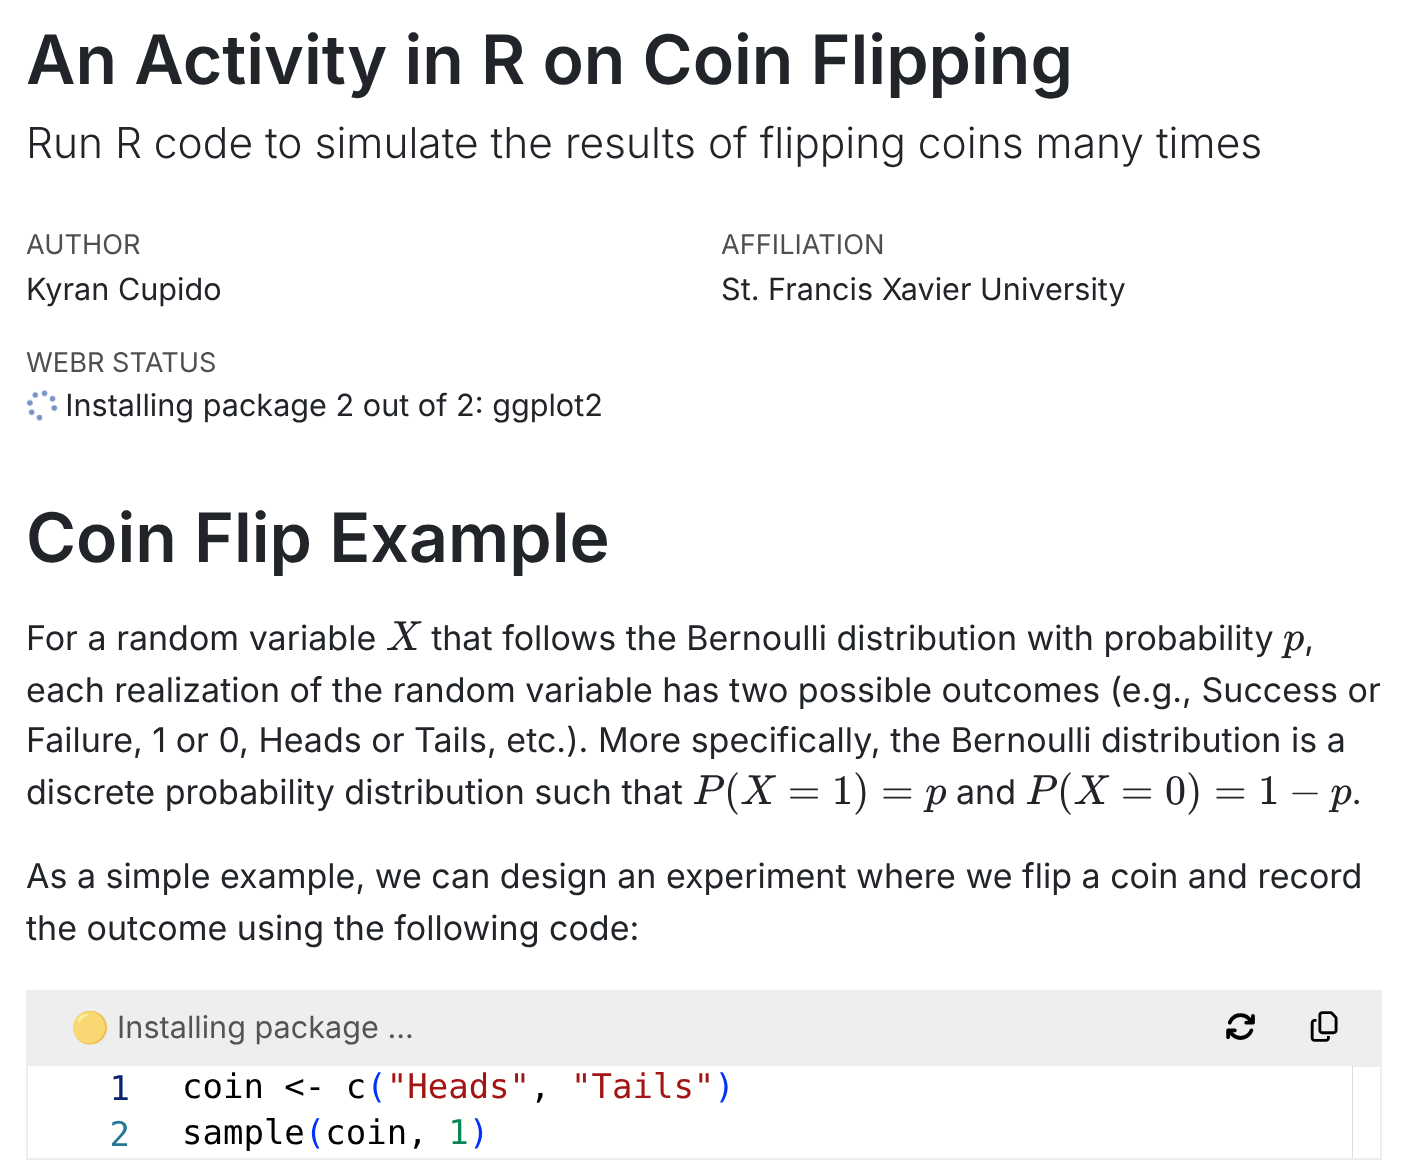
\includegraphics[keepaspectratio]{figures/fig-webr-loading.png}}

}

\subcaption{\label{fig-loading-a}While loading}

\end{minipage}%
%
\begin{minipage}{0.50\linewidth}

\centering{

\pandocbounded{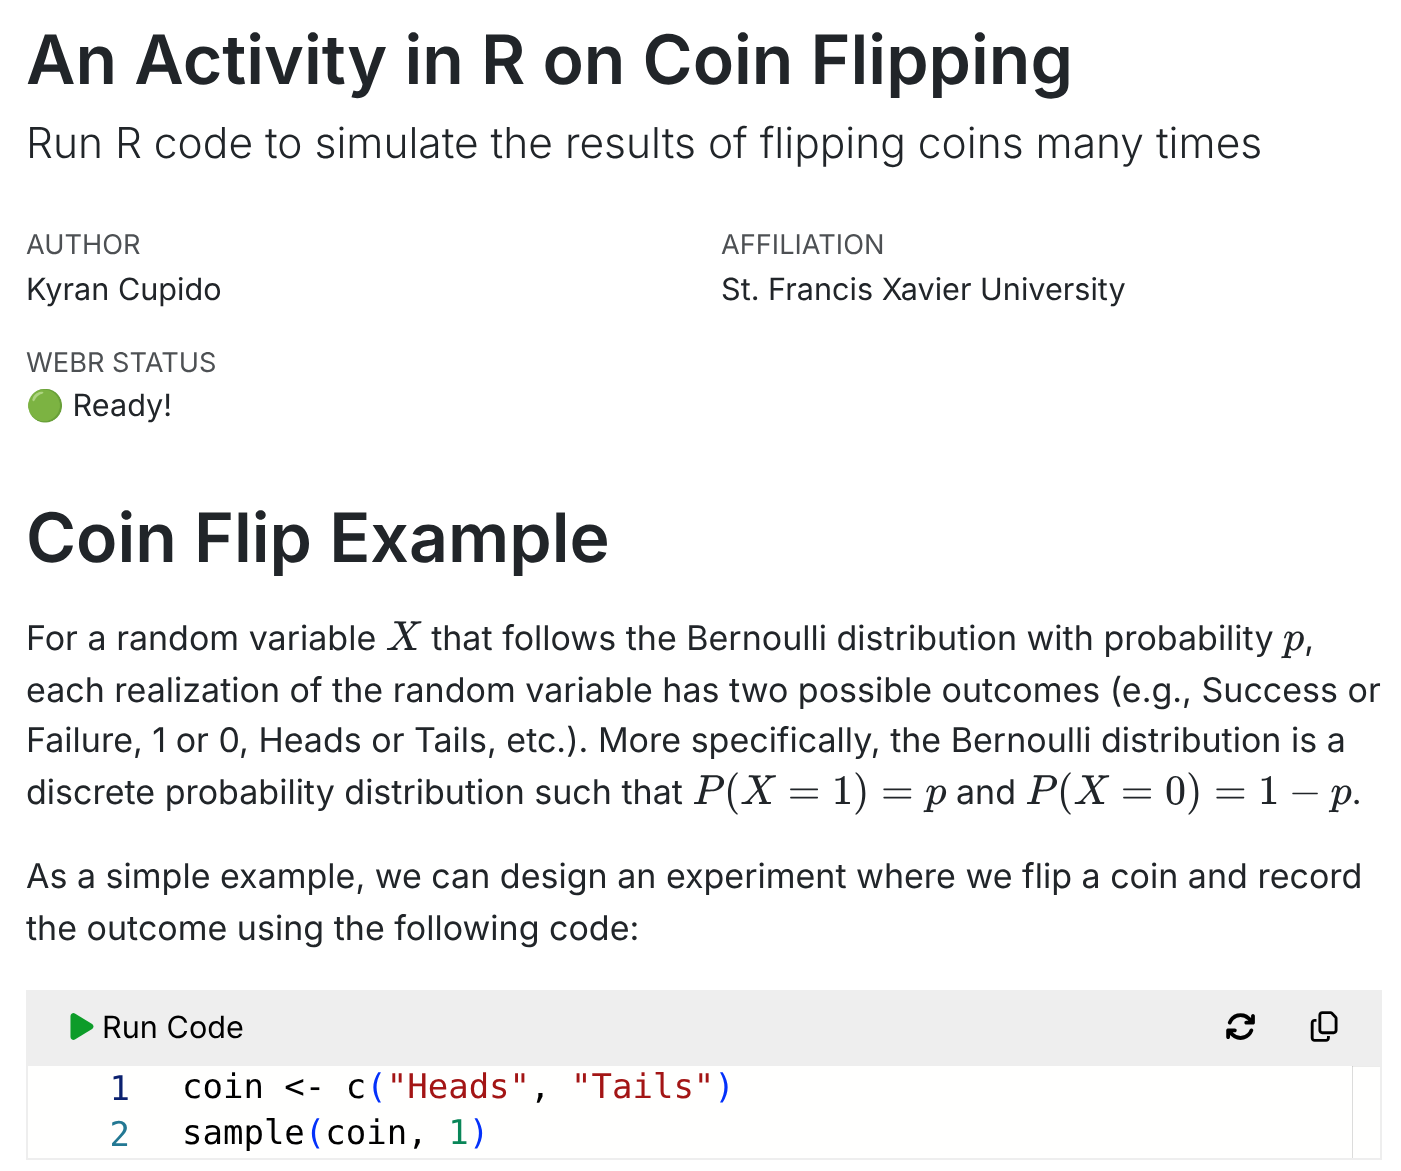
\includegraphics[keepaspectratio]{figures/fig-webr-ready.png}}

}

\subcaption{\label{fig-loading-b}Ready}

\end{minipage}%

\caption{\label{fig-loading}The coin-flipping activity (a) while webR
installs the declared packages and (b) once the R session is ready.}

\end{figure}%

\subsection{Structure of the template}\label{sec-webr-structure}

The landing page (Figure~\ref{fig-landing}) links to the syllabus and to
schedules of lecture slides, activities and tutorials. Each item is a
separate Quarto document, so weeks are added or removed by editing a
table.

\begin{figure}[H]

\centering{

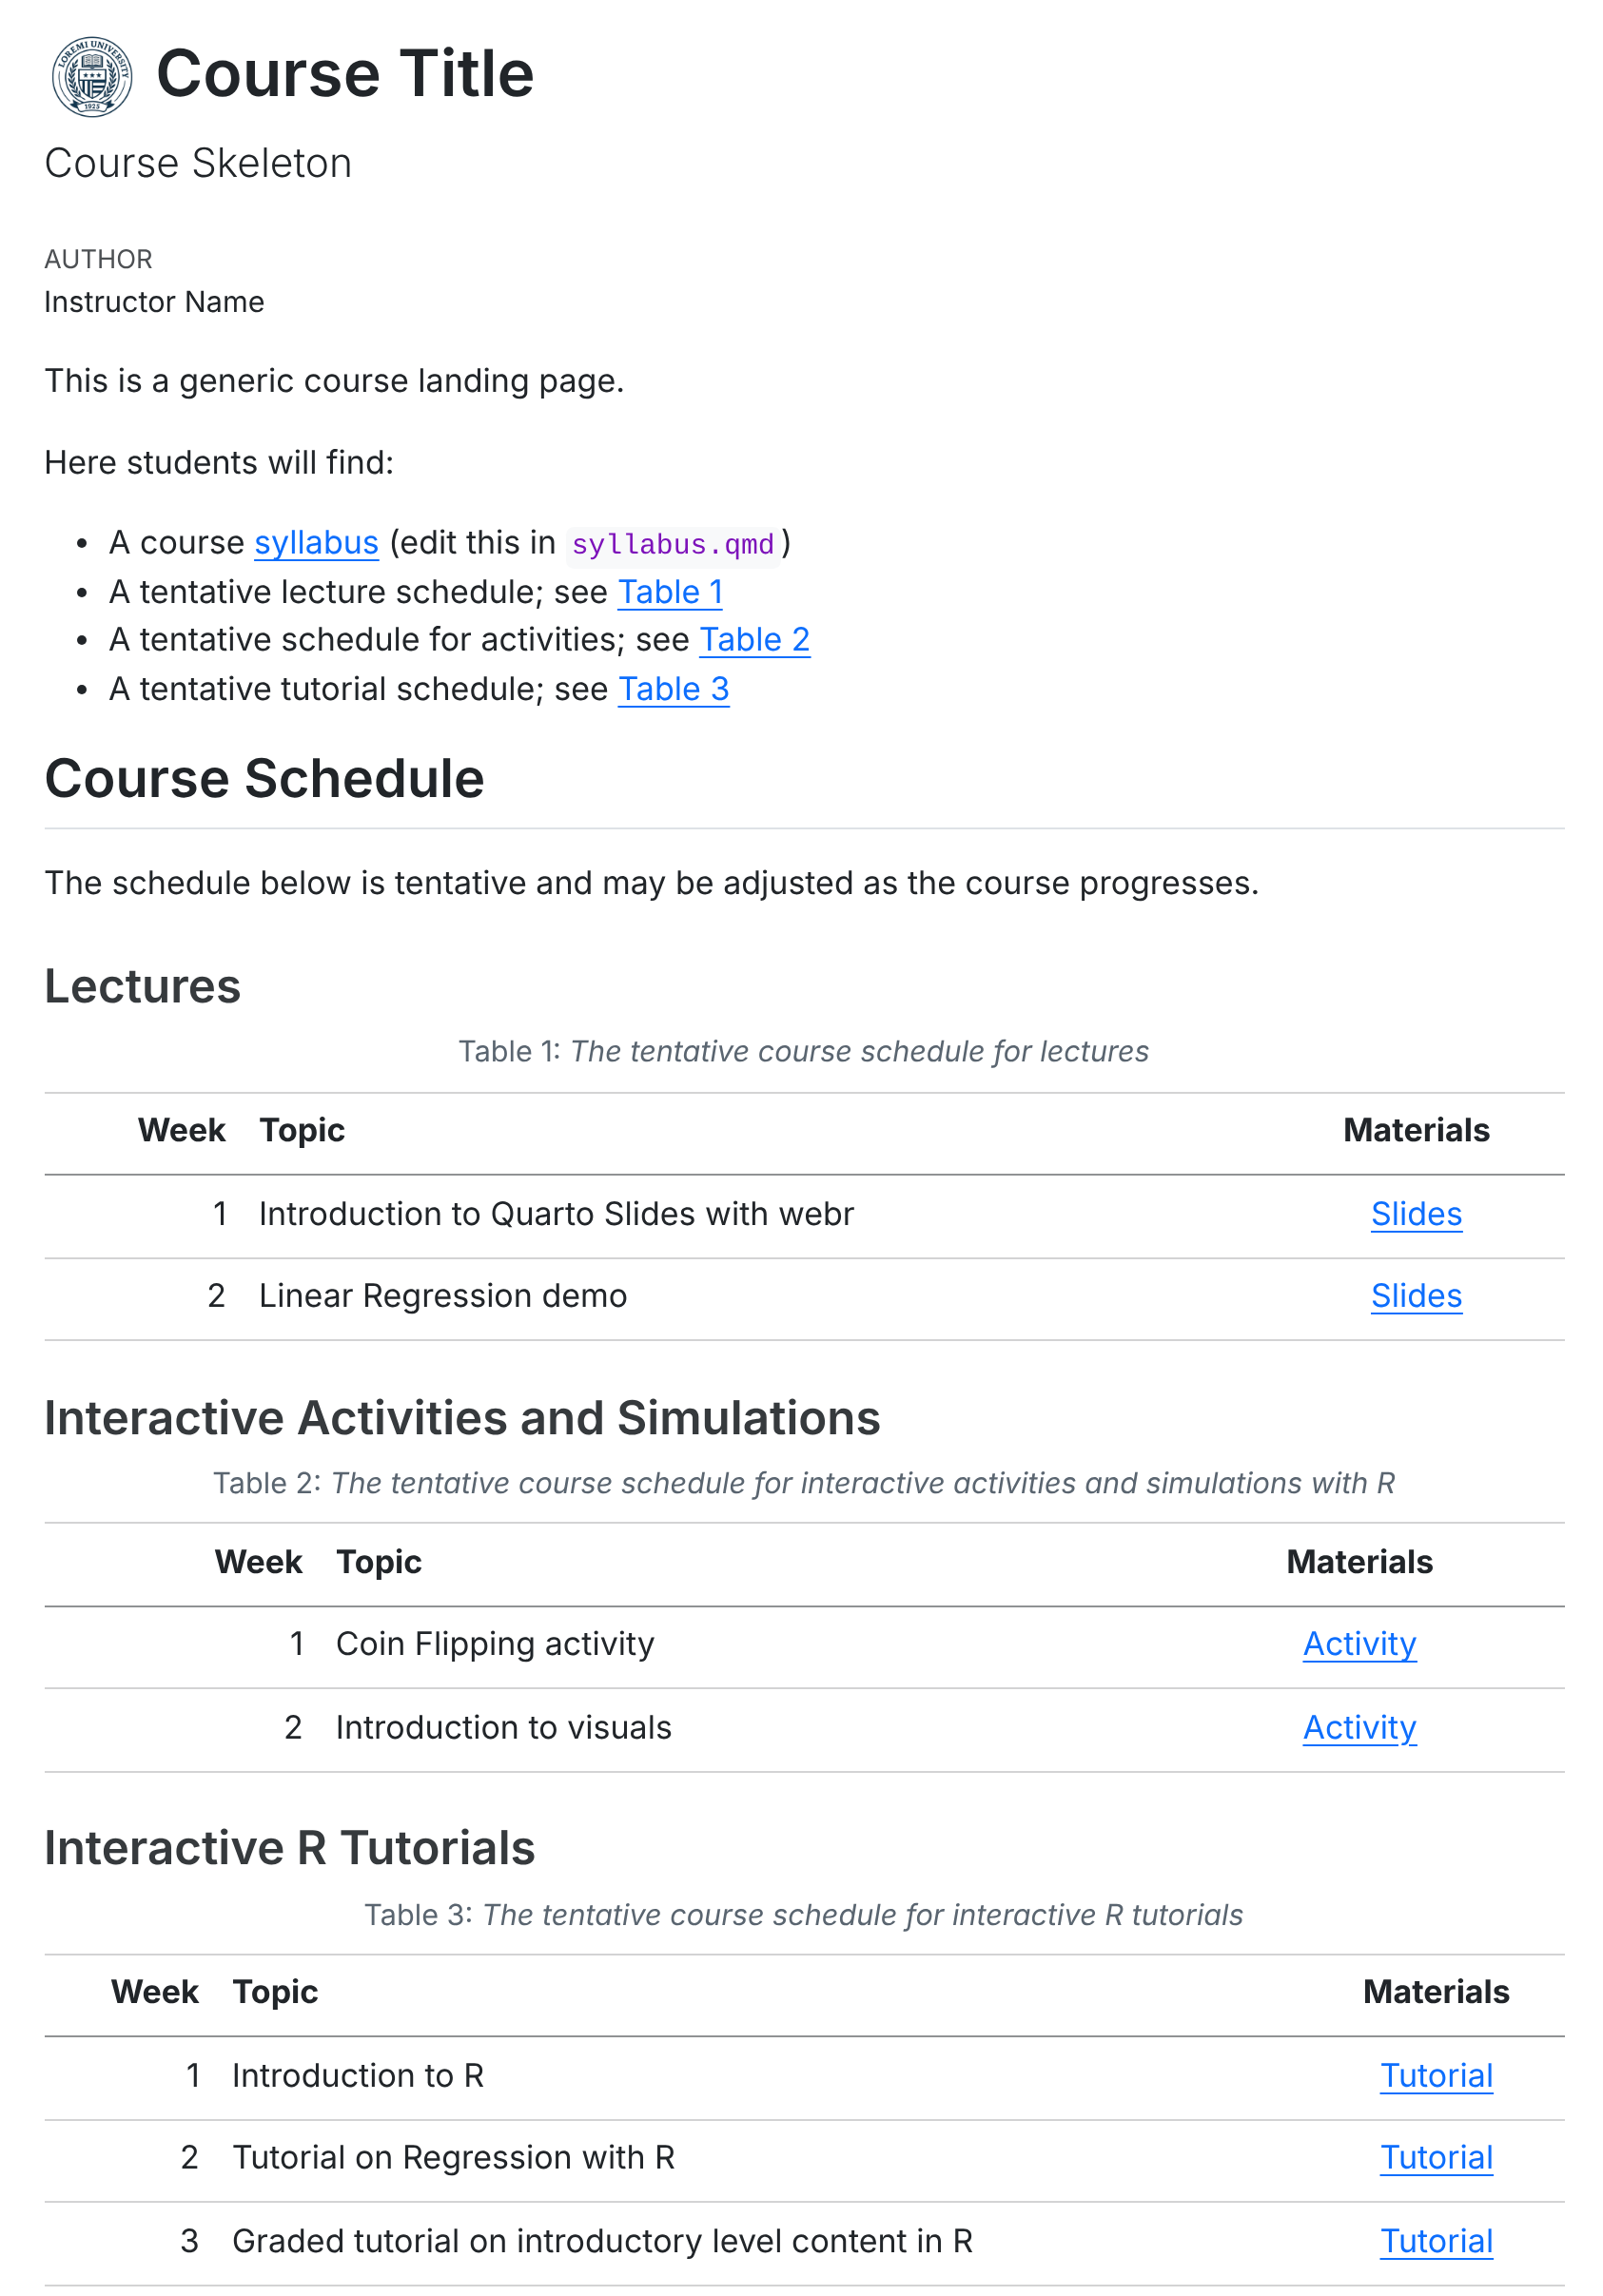
\includegraphics[width=0.65\linewidth,height=\textheight,keepaspectratio]{figures/fig-landing.png}

}

\caption{\label{fig-landing}Landing page of the course skeleton.}

\end{figure}%

\textbf{Lecture slides.} The slides are revealjs presentations with
embedded \texttt{\{webr-r\}} cells, which allow code to be run and
modified during the lecture without leaving the slides
(Figure~\ref{fig-slide}). The same deck can be printed to PDF.

\begin{figure}[H]

\centering{

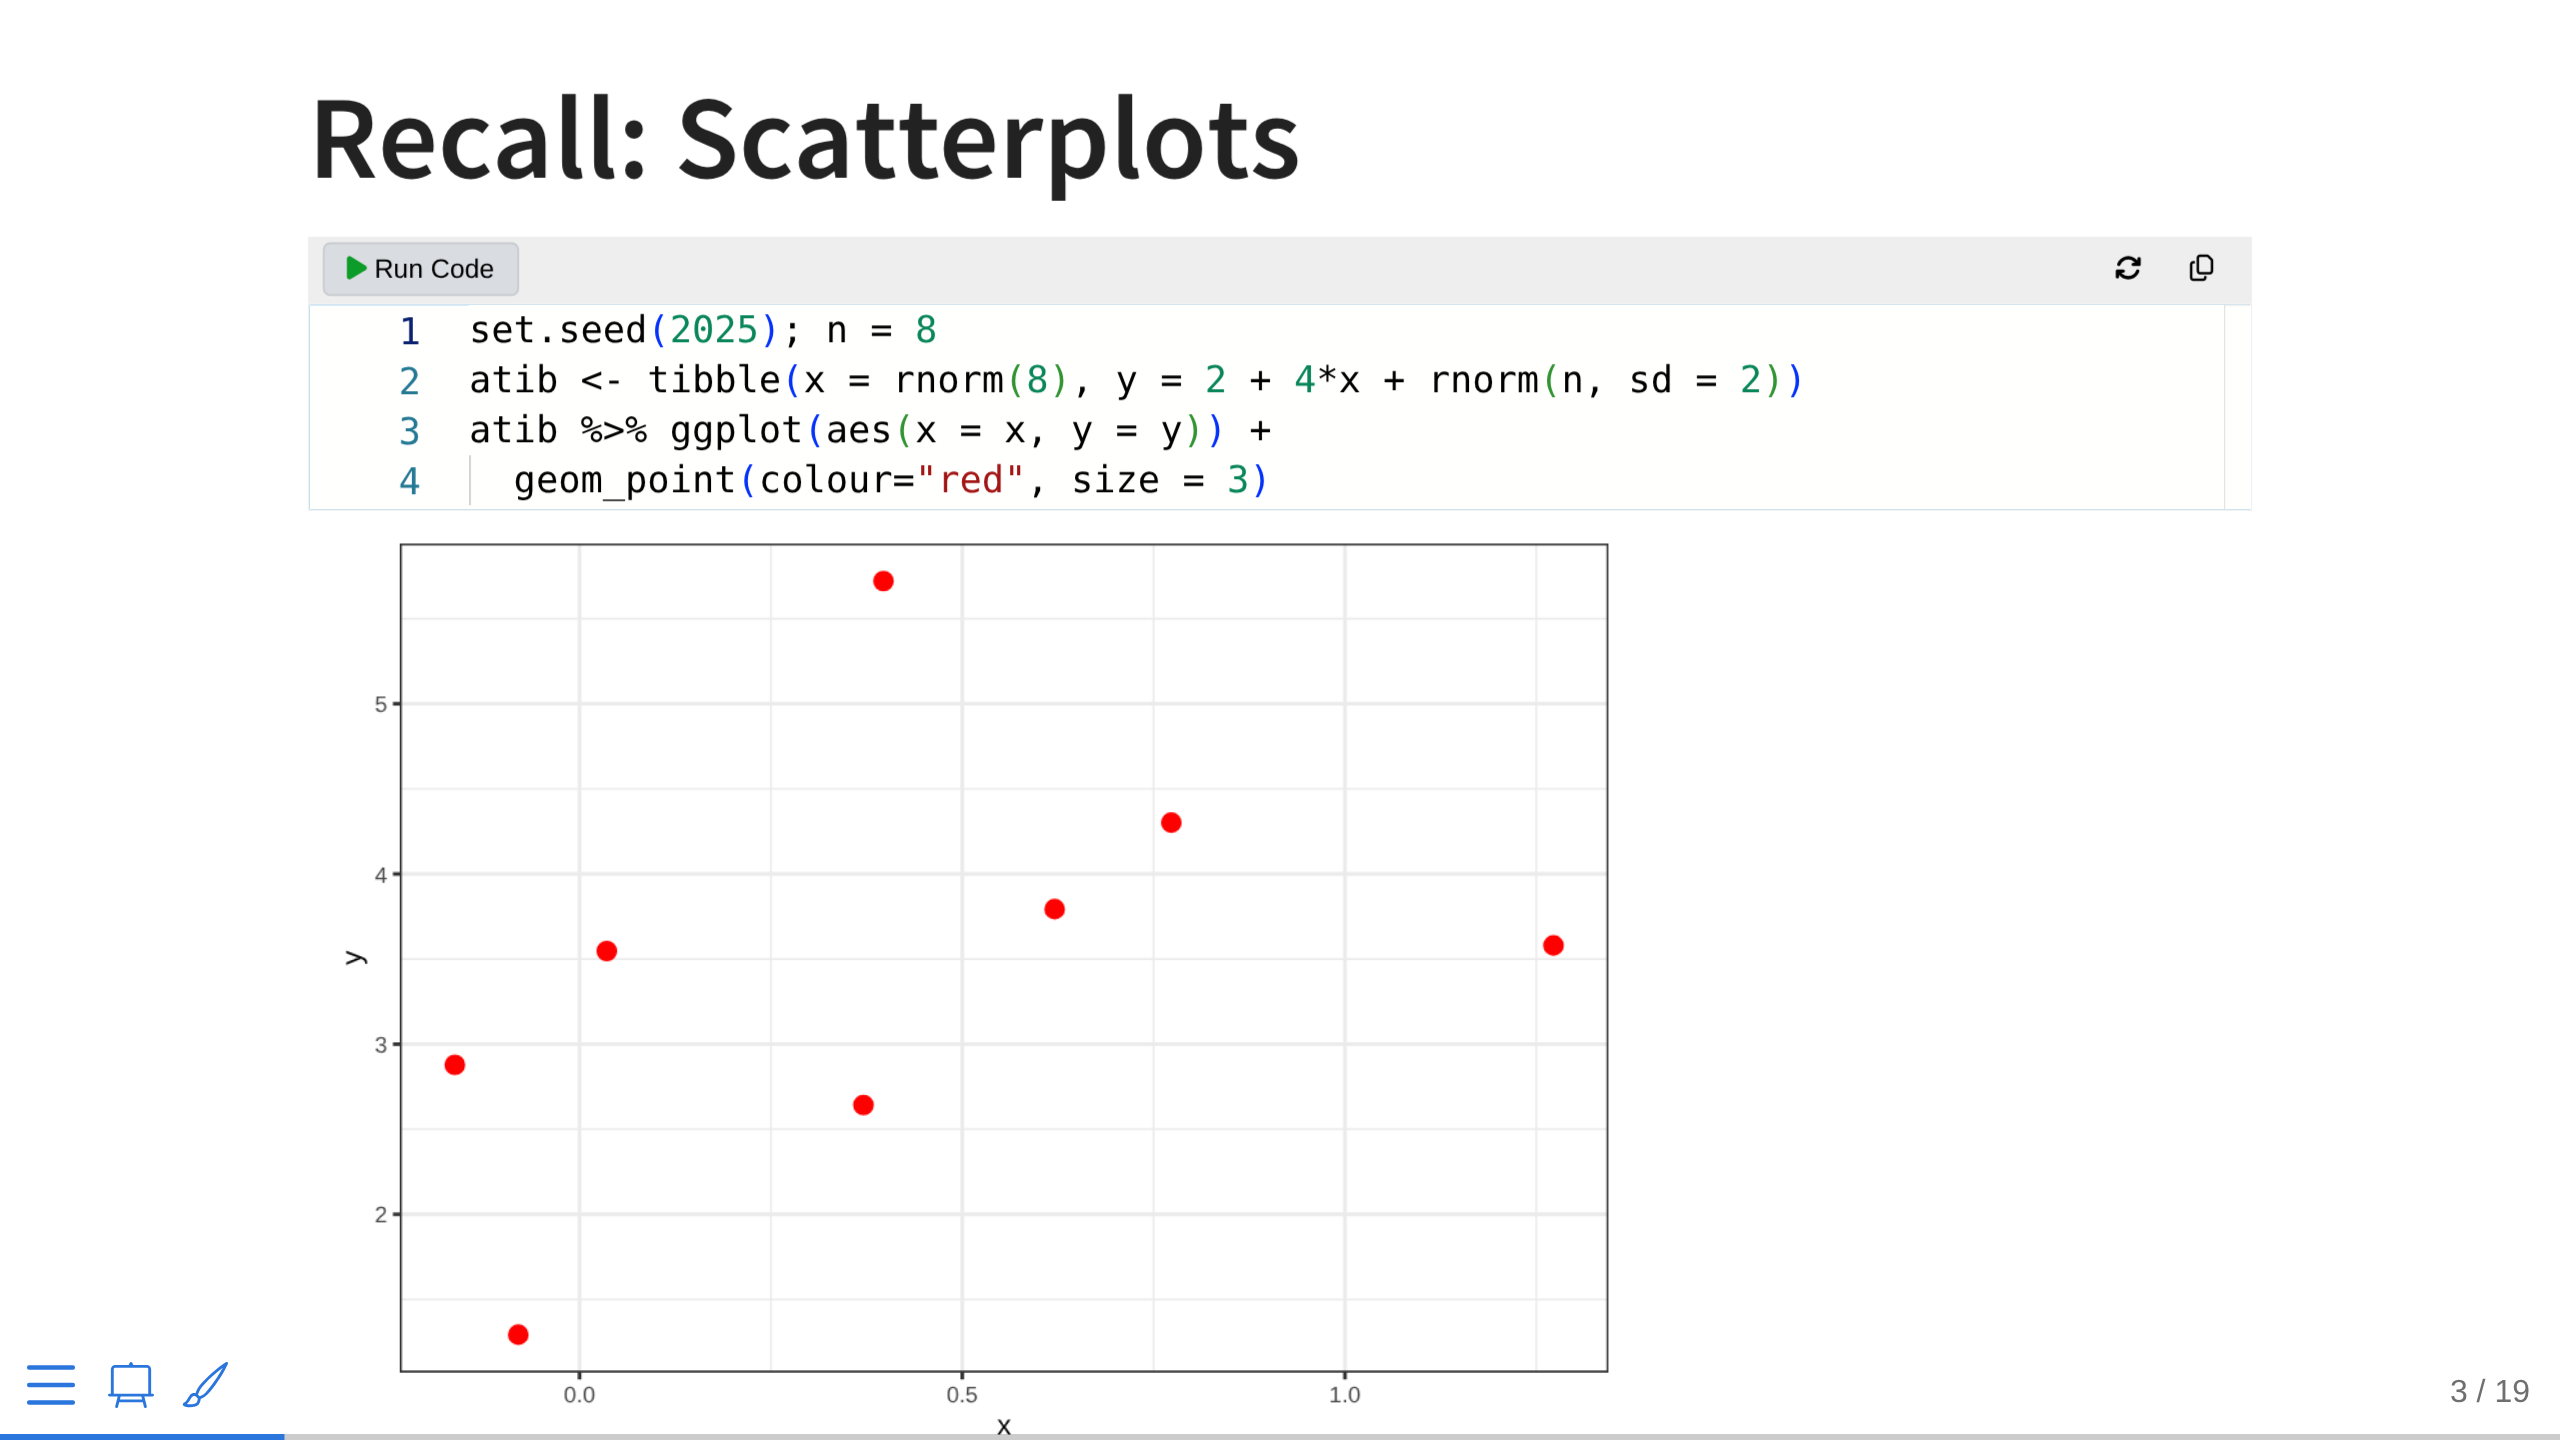
\includegraphics[width=0.8\linewidth,height=\textheight,keepaspectratio]{figures/fig-slide-webr.png}

}

\caption{\label{fig-slide}A slide from the regression lecture after
running the code. Tall plots may be cut off at the bottom of the slide,
as is the case for the \(x\)-axis label here.}

\end{figure}%

\textbf{Activities and simulations.} Activities combine short
explanations with code cells that students modify and re-run. The
coin-flipping activity builds up to a simulation of the running
proportion of heads (Figure~\ref{fig-activity-a}), and the Pixar
activity uses the \texttt{pixarfilms} package for descriptive statistics
and basic graphs (Figure~\ref{fig-activity-b}).

\begin{figure}[H]

\begin{minipage}{0.47\linewidth}

\centering{

\pandocbounded{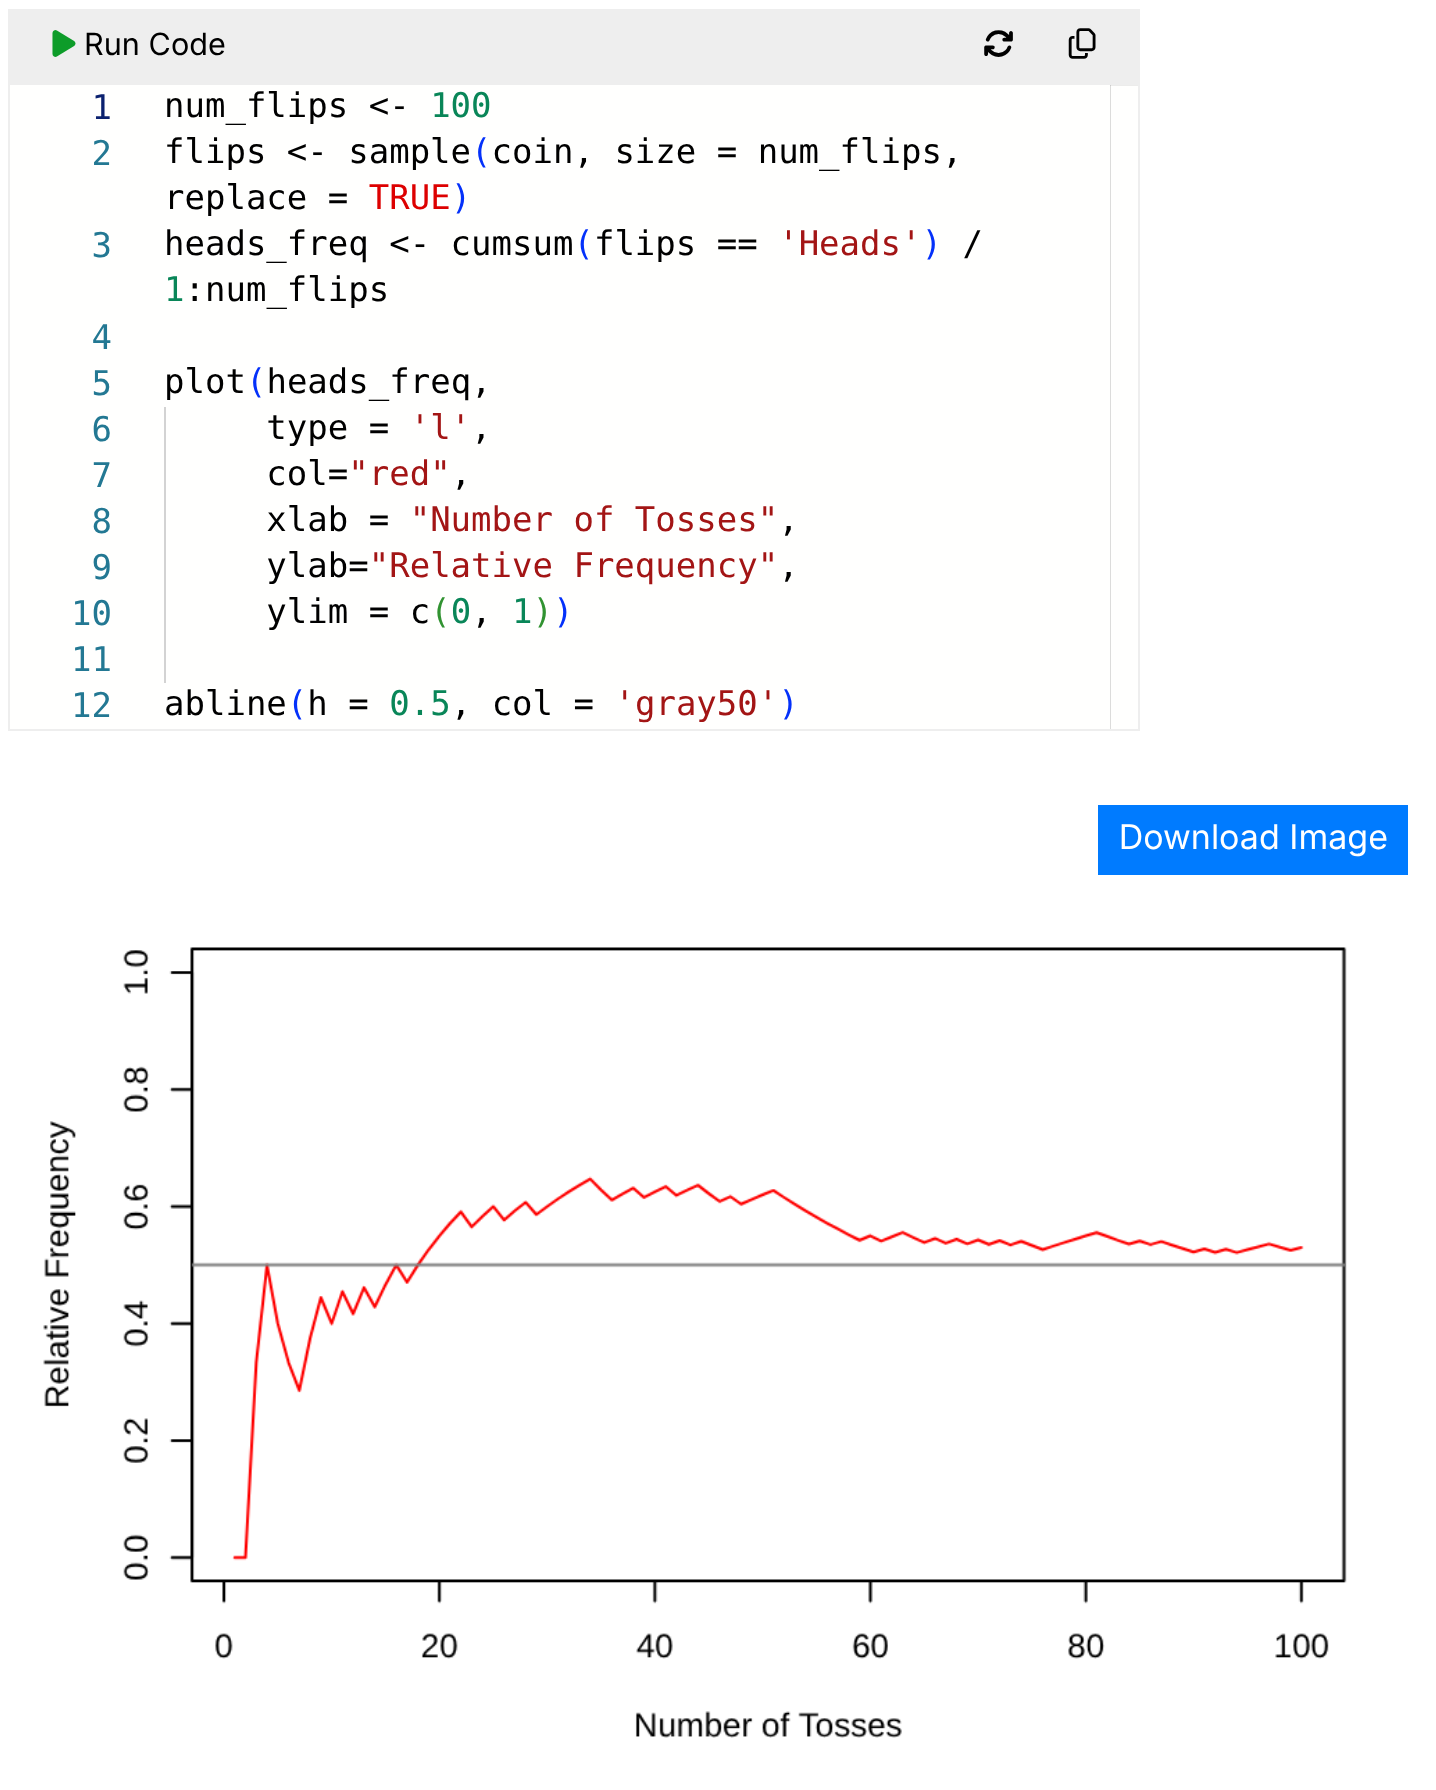
\includegraphics[keepaspectratio]{figures/fig-activity-coins.png}}

}

\subcaption{\label{fig-activity-a}Coin flipping}

\end{minipage}%
%
\begin{minipage}{0.53\linewidth}

\centering{

\pandocbounded{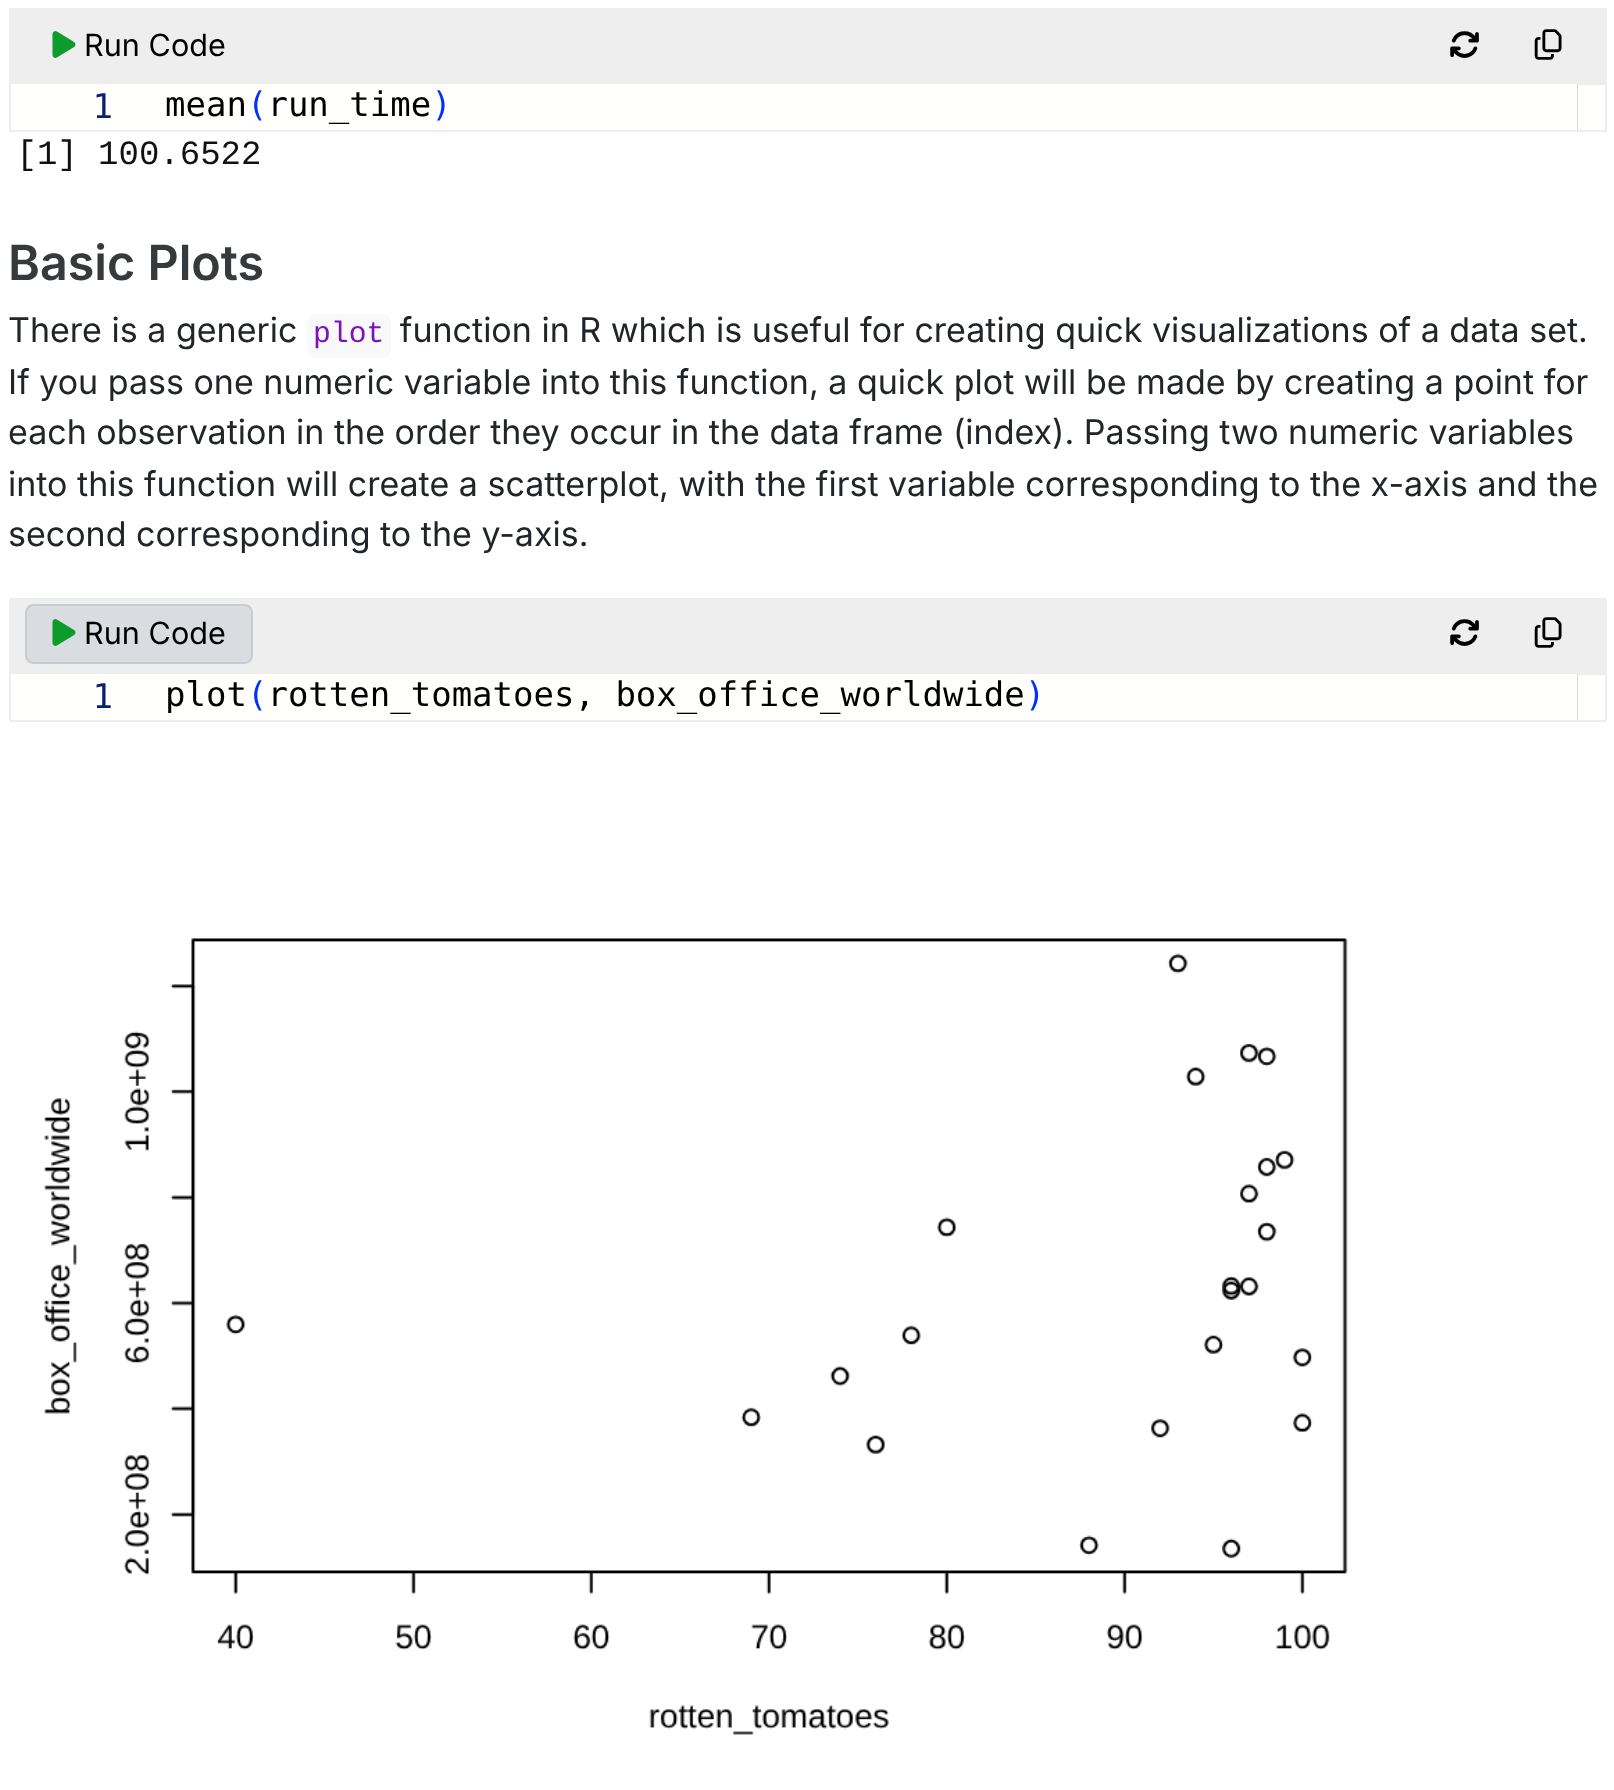
\includegraphics[keepaspectratio]{figures/fig-activity-pixar.png}}

}

\subcaption{\label{fig-activity-b}Pixar films}

\end{minipage}%

\caption{\label{fig-activity}Code cells from the two activities after
running the code.}

\end{figure}%

\textbf{Tutorials.} The ungraded tutorials follow a worked-example
format. In the regression tutorial, students explore the Palmer penguins
data \citep{palmerpenguins} and fit a simple linear regression with
\texttt{lm()} (Figure~\ref{fig-tutorial}). The R session persists across
the cells of a page, as in an ordinary R script.

\begin{figure}[H]

\centering{

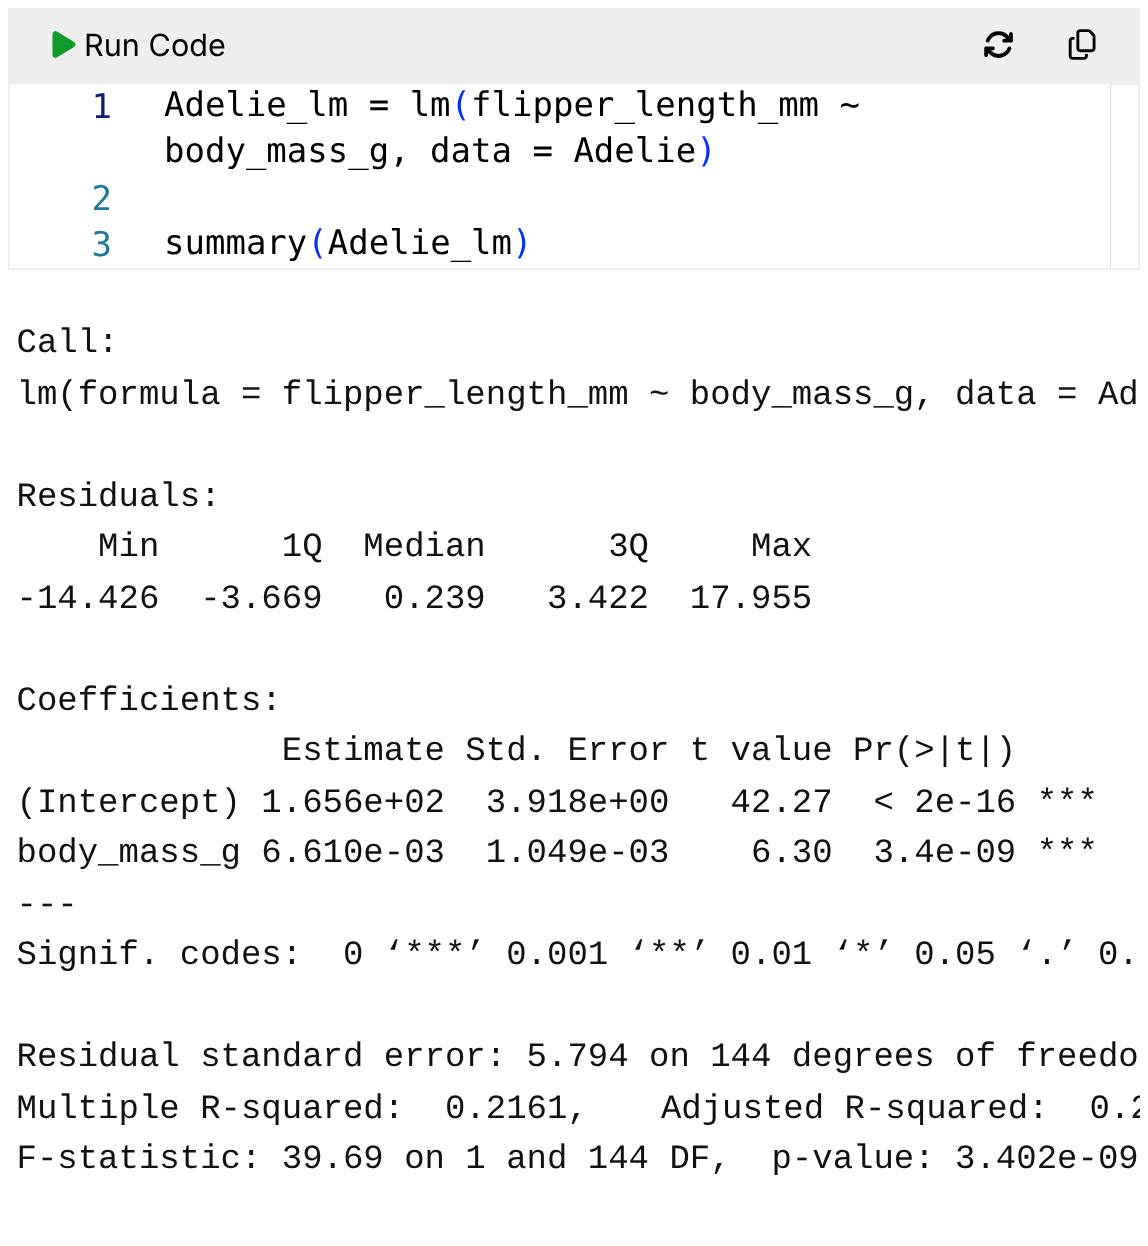
\includegraphics[width=0.55\linewidth,height=\textheight,keepaspectratio]{figures/fig-regression-lm.png}

}

\caption{\label{fig-tutorial}A cell from the regression tutorial. Long
output lines are truncated at the edge of the cell.}

\end{figure}%

\subsection{Example of use: graded exercises}\label{sec-webr-exercises}

Each exercise in the graded tutorial consists of up to five chunks that
share an \texttt{exercise} label: an optional setup chunk, the starting
code, a hint, a model solution and a check. Listing~\ref{lst-ex-sum}
shows the source of the first exercise, which asks students to replace
two blanks so that an expression evaluates to 10. The blanks are written
with a full-width underscore character (＿), which the setup chunk
defines as a missing value.

\begin{codelisting}

\caption{\label{lst-ex-sum}Quarto source of the first exercise of the
graded tutorial, consisting of a setup chunk, the starting code, a hint,
a model solution and a check written with gradethis.}

\centering{

\begin{Shaded}
\begin{Highlighting}[]
\InformationTok{\textasciigrave{}\textasciigrave{}\textasciigrave{}\{webr\}}
\InformationTok{\#| setup: true}
\InformationTok{\#| exercise: ex\_sum}
\InformationTok{＿ \textless{}{-} NA\_real\_}
\InformationTok{\textasciigrave{}\textasciigrave{}\textasciigrave{}}

\InformationTok{\textasciigrave{}\textasciigrave{}\textasciigrave{}\{webr\}}
\InformationTok{\#| exercise: ex\_sum}
\InformationTok{1 + 2 + ＿ + ＿}
\InformationTok{\textasciigrave{}\textasciigrave{}\textasciigrave{}}

\NormalTok{::: \{.hint exercise="ex\_sum"\}}
\NormalTok{Replace the two ＿ with 2 numbers that add up to 7.}
\NormalTok{:::}

\NormalTok{::: \{.solution exercise="ex\_sum"\}}
\InformationTok{\textasciigrave{}\textasciigrave{}\textasciigrave{}\{webr\}}
\InformationTok{\#| exercise: ex\_sum}
\InformationTok{\#| solution: true}
\InformationTok{1 + 2 + 3 + 4}
\InformationTok{\textasciigrave{}\textasciigrave{}\textasciigrave{}}
\NormalTok{:::}

\InformationTok{\textasciigrave{}\textasciigrave{}\textasciigrave{}\{webr\}}
\InformationTok{\#| exercise: ex\_sum}
\InformationTok{\#| check: true}
\InformationTok{gradethis::grade\_this(\{}
\InformationTok{  if (grepl("＿", .user\_code, fixed = TRUE)) \{}
\InformationTok{    fail("Replace ＿ with a number.")}
\InformationTok{  \}}
\InformationTok{  if (is.numeric(.result) \&\& length(.result) == 1 \&\&}
\InformationTok{      isTRUE(all.equal(.result, 10))) \{}
\InformationTok{    pass("✅ Correct!")}
\InformationTok{  \} else \{}
\InformationTok{    fail("Not quite — try to make the expression evaluate to 10.")}
\InformationTok{  \}}
\InformationTok{\})}
\InformationTok{\textasciigrave{}\textasciigrave{}\textasciigrave{}}
\end{Highlighting}
\end{Shaded}

}

\end{codelisting}%

Within \texttt{grade\_this()}, the check has access to the student's
code as text (\texttt{.user\_code}), the value of the last expression
(\texttt{.result}) and the evaluation environment
(\texttt{.envir\_result}), and returns feedback through \texttt{pass()}
or \texttt{fail()}. Checks are therefore ordinary R code. Running the
code displays its output followed by the feedback from the check
(Figure~\ref{fig-exercise}). Once the hint has been revealed, the hint
button is replaced by a ``Show Solution'' button, so that assistance is
provided in stages.

\begin{figure}[H]

\begin{minipage}{\linewidth}

\centering{

\pandocbounded{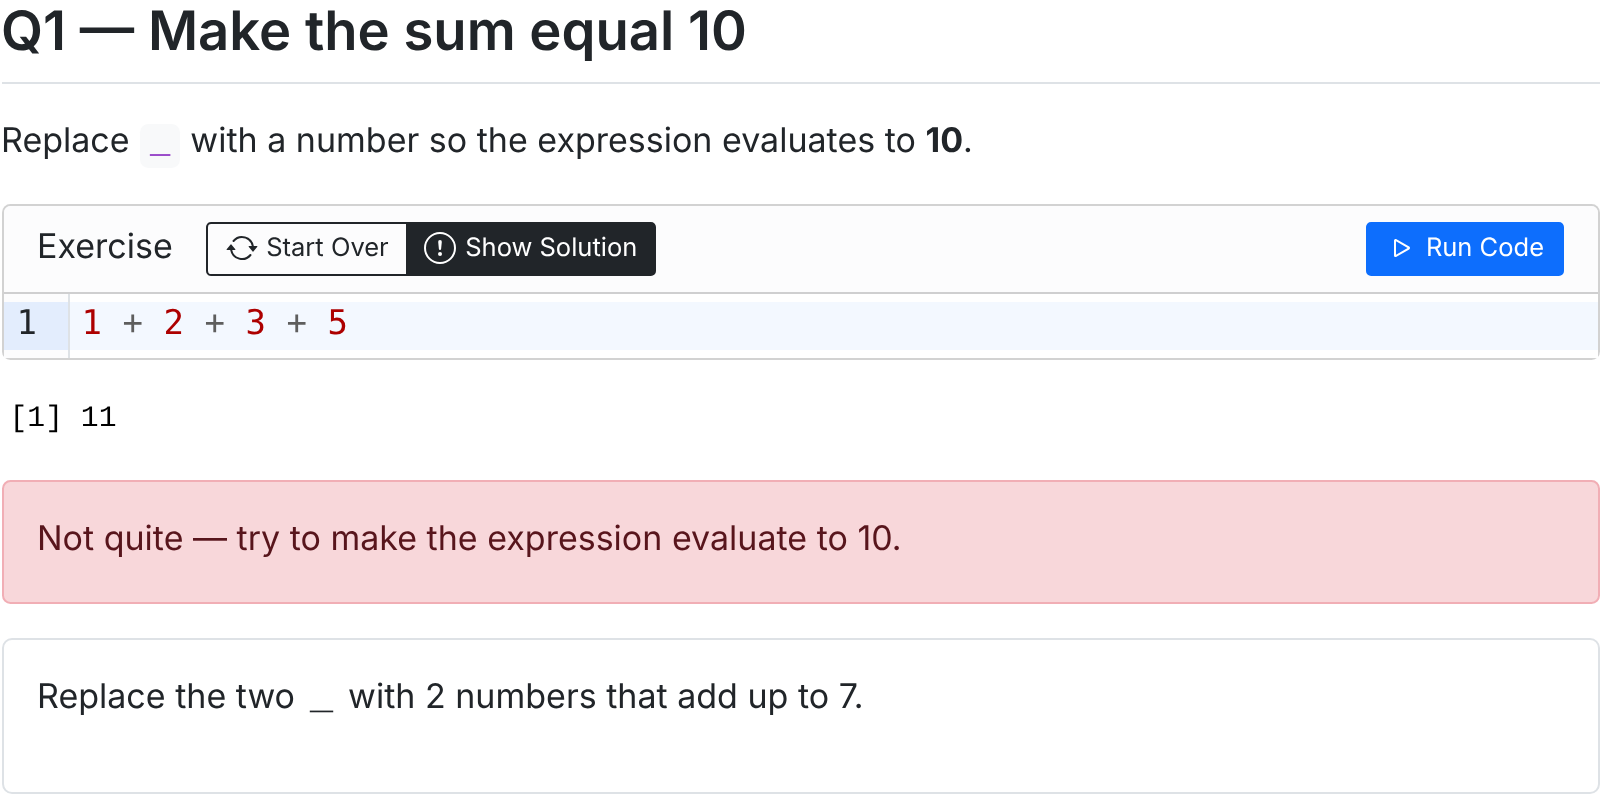
\includegraphics[keepaspectratio]{figures/fig-ex-fail-hint.png}}

}

\subcaption{\label{fig-exercise-a}Incorrect answer, after revealing the
hint}

\end{minipage}%
\newline
\begin{minipage}{\linewidth}

\centering{

\pandocbounded{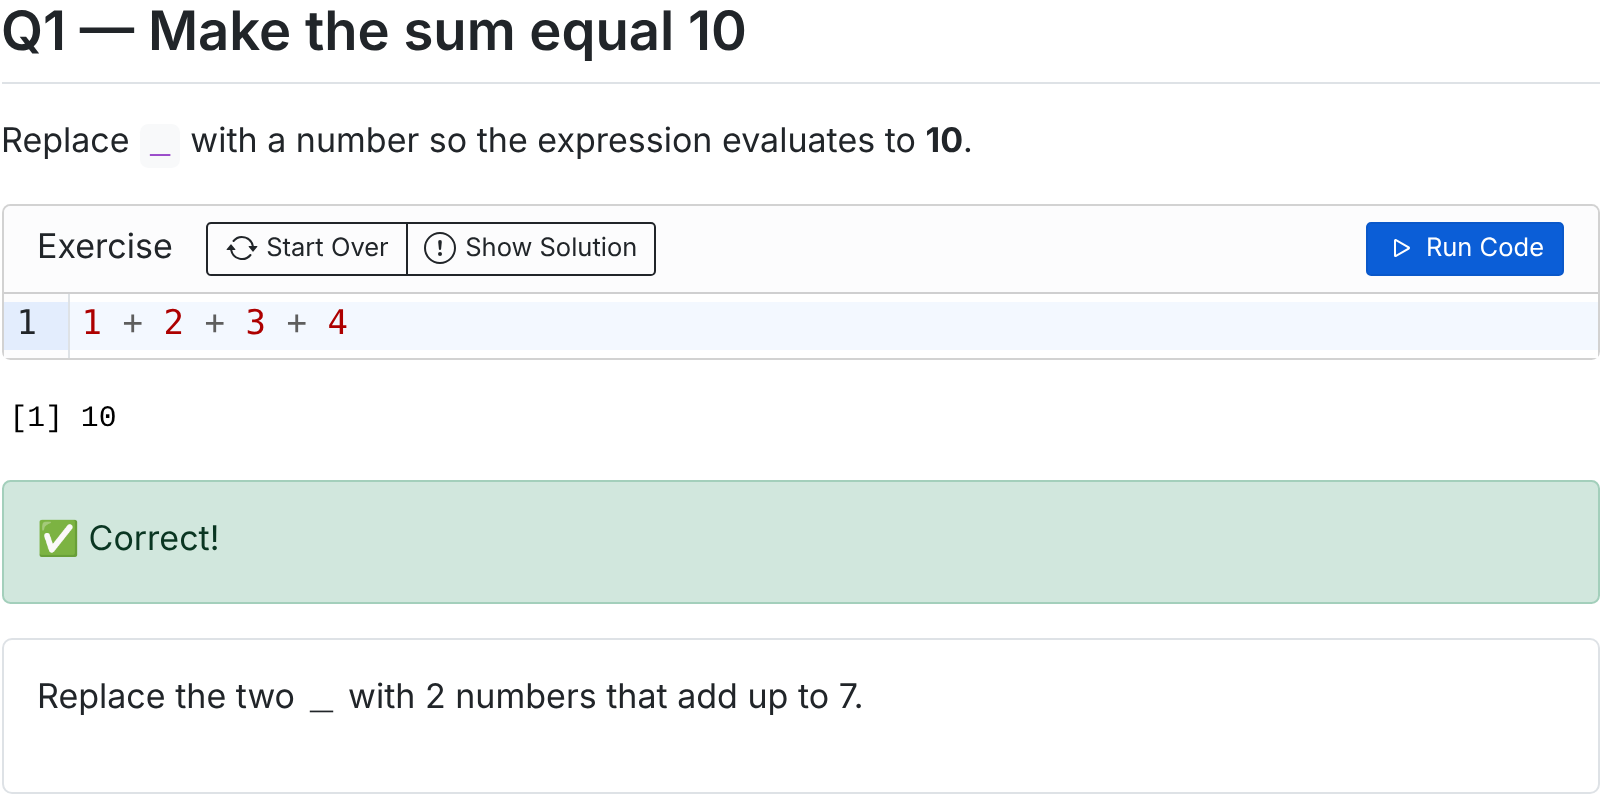
\includegraphics[keepaspectratio]{figures/fig-ex-pass.png}}

}

\subcaption{\label{fig-exercise-b}Correct answer}

\end{minipage}%

\caption{\label{fig-exercise}The first exercise of the graded tutorial,
with (a) an incorrect answer and the hint and (b) the corrected answer.}

\end{figure}%

Later exercises inspect the code itself. For a question requiring a
histogram of one column of \texttt{ToothGrowth}, the check parses the
submission with \texttt{parse()} and verifies that it is a single call
to \texttt{hist()} with an admissible argument, which allows targeted
messages for anticipated mistakes (Figure~\ref{fig-solution}). R errors
are displayed in the cell as in an ordinary R session
(Figure~\ref{fig-error}).

\begin{figure}[H]

\centering{

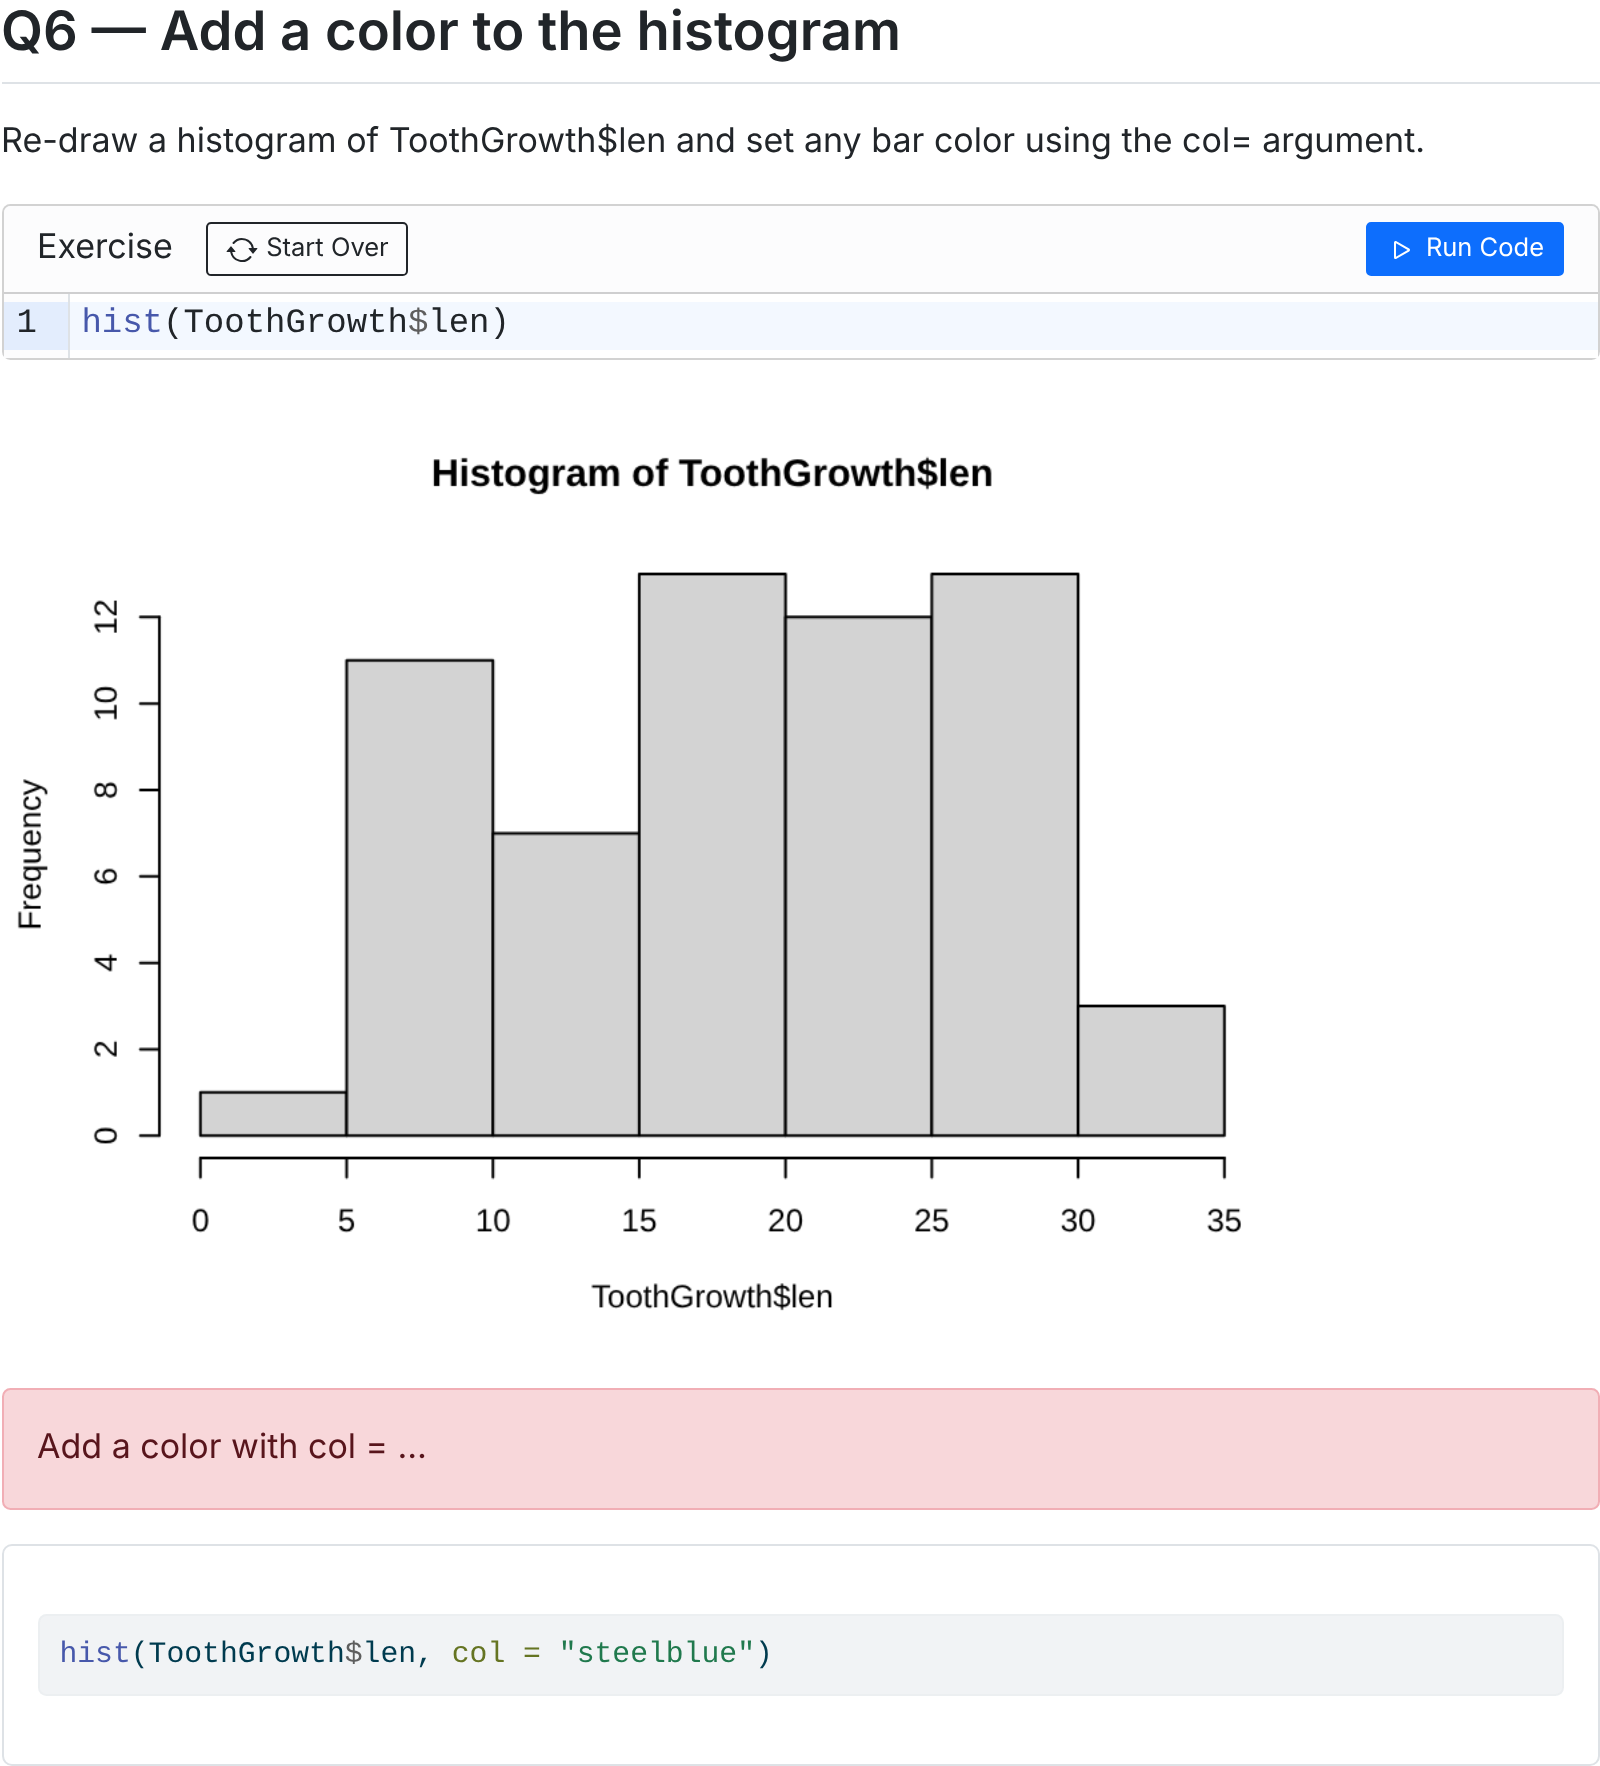
\includegraphics[width=0.65\linewidth,height=\textheight,keepaspectratio]{figures/fig-ex-solution.png}

}

\caption{\label{fig-solution}An exercise in which the check detects a
missing \texttt{col} argument, followed by the hint and the solution.}

\end{figure}%

\begin{figure}[H]

\centering{

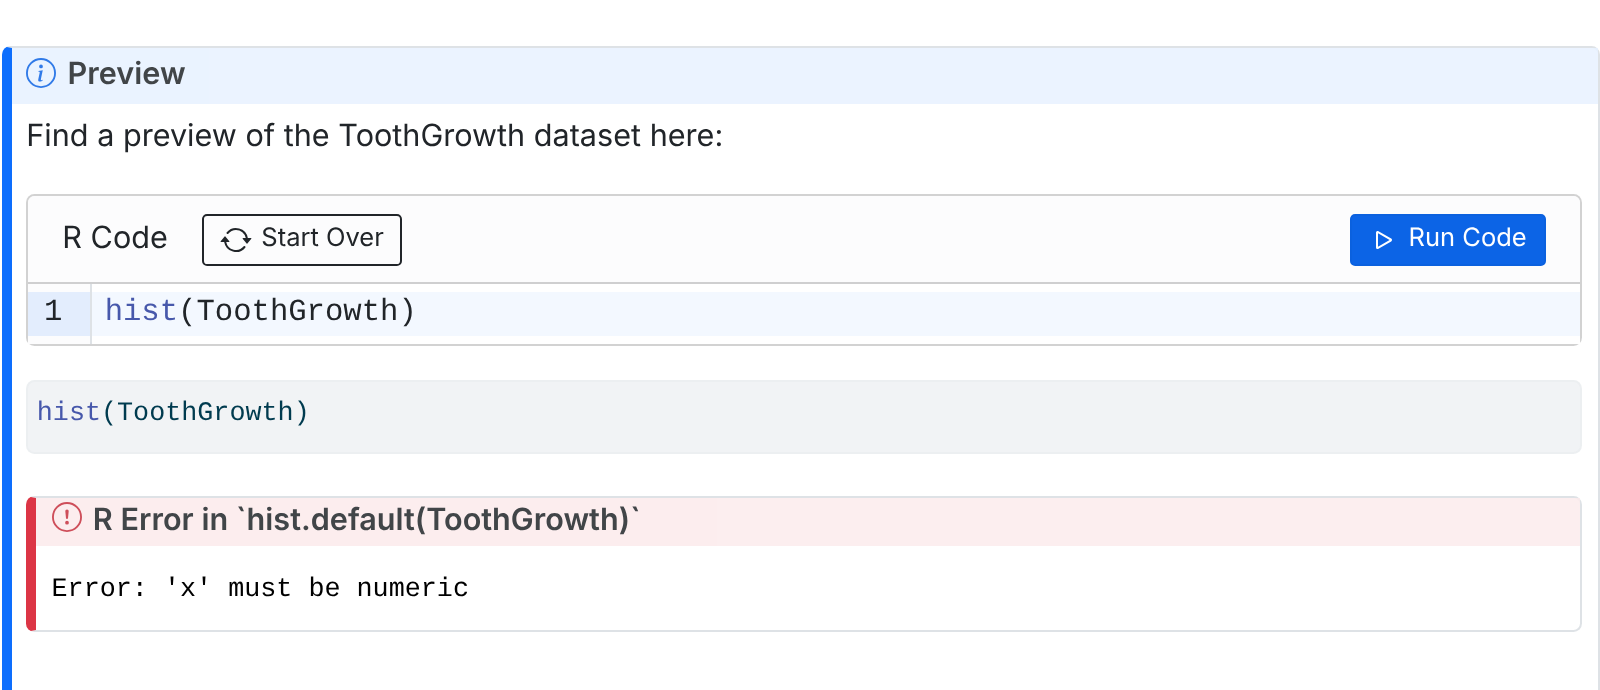
\includegraphics[width=0.65\linewidth,height=\textheight,keepaspectratio]{figures/fig-ex-error.png}

}

\caption{\label{fig-error}An R error displayed in an interactive cell of
the graded tutorial.}

\end{figure}%

Checks may also be too permissive. The third exercise asks for the mean
of \texttt{c(2,\ 4,\ 6,\ 8,\ 10)}, but the check only compares the
stored value with 6, so the median of a different vector is accepted
(Figure~\ref{fig-false-positive}). Checks that compare values should
therefore anticipate incorrect approaches, for instance by also
inspecting the code for a call to \texttt{mean()}; we return to this
point in Section~\ref{sec-design}.

\begin{figure}[H]

\centering{

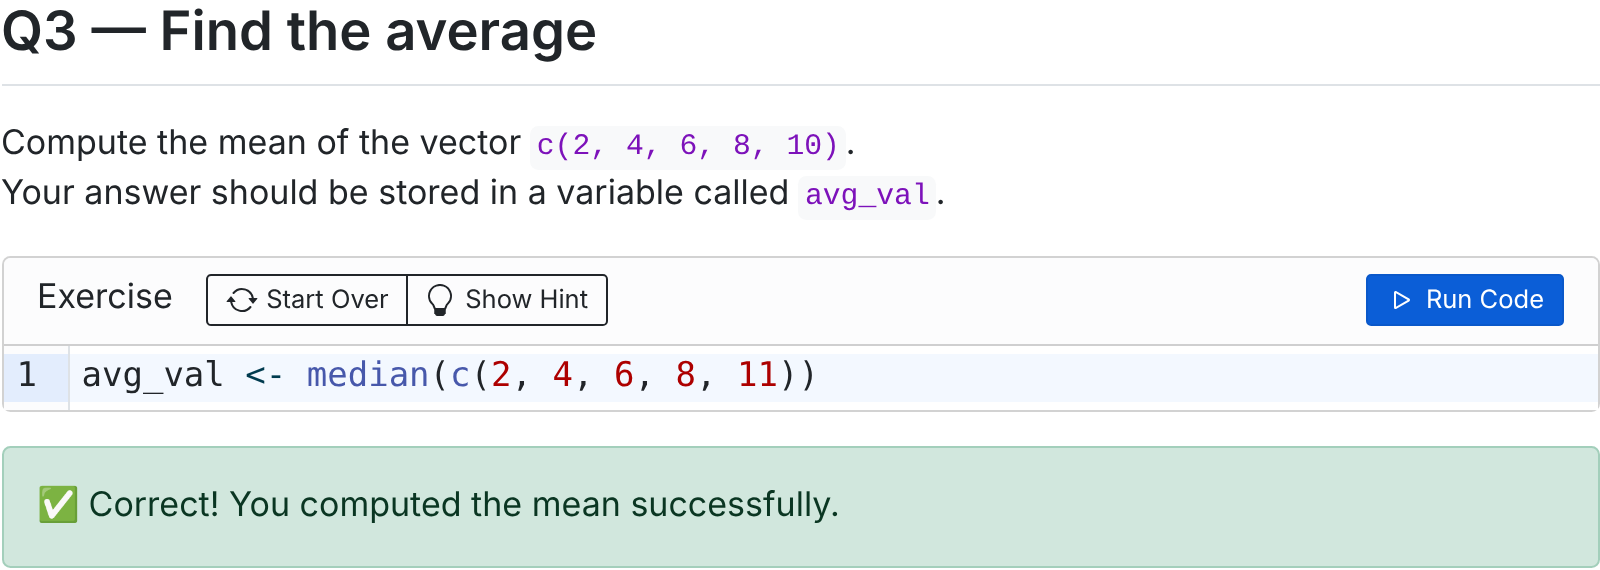
\includegraphics[width=0.65\linewidth,height=\textheight,keepaspectratio]{figures/fig-ex-false-positive.png}

}

\caption{\label{fig-false-positive}A false positive: an answer based on
the median of a different vector is accepted because only the final
value is checked.}

\end{figure}%

\section{Strengths and limitations of the webR
approach}\label{sec-strengths}

The main strength of the approach is that students can run R without
installing software, which removes a frequent source of difficulty at
the start of a course and on restricted machines. Instructors write
materials in Quarto or R Markdown, a single source can produce slides,
notes and exercises, and hosting is free and requires no server
administration. Exercises provide immediate feedback, and since checks
are written in R, the feedback can be tailored to anticipated mistakes.
The approach is therefore well suited to live demonstrations, in-class
activities and simulations, pre-lab preparation and low-stakes
self-assessment.

Without additional infrastructure, the approach has the following
limitations.

\begin{itemize}
\tightlist
\item
  \emph{Summative assessment.} Solutions are embedded in the page
  source, and the checks are sent to the browser, where grading takes
  place. Students who inspect the page can therefore obtain the answers.
\item
  \emph{Recording student work.} Results are displayed to the student
  but are neither stored nor transmitted to the instructor, and there is
  no integration with a learning management system.
\item
  \emph{Persistence.} In our tests, edits to exercises were lost when
  the page was reloaded.
\item
  \emph{Packages and computation.} Only packages with WebAssembly builds
  are available, and computations run on the student's device, which
  limits the size of data and the computational load.
\item
  \emph{Interactive features.} On hosts that do not send specific HTTP
  headers, such as GitHub Pages, functions requiring keyboard input
  (e.g., \texttt{readline()} or the debugger) are unavailable.
\item
  \emph{Layout.} Wide output may be truncated
  (Figure~\ref{fig-tutorial}) and tall plots may overflow slides
  (Figure~\ref{fig-slide}).
\item
  \emph{Maturity.} webR and both extensions are under active development
  \citep{webRdocs}, and the two extensions use different chunk syntax.
\end{itemize}

\section{\texorpdfstring{Interactive tutorials for learning and
assessment using
\texttt{learnR}}{Interactive tutorials for learning and assessment using learnR}}\label{sec-learnr}

\subsection{Main initial takeaways}\label{main-initial-takeaways}

\begin{itemize}
\tightlist
\item
  Best use is for interactive, low stakes tutorials.
\item
  Supports active learning since students learn by running code.
\item
  Good for formative assessment: useful for practice, readiness checks,
  lab prep, and review rather than formal high-stakes grading.
\item
  Works best for smaller code tasks to simplify feedback through
  \texttt{gradethis}.
\item
  Immediate feedback is available with \texttt{gradethis}.
\item
  Student work can be tracked easily through \texttt{learnrhash}, as
  long as you need an existence proof and not a formal evaluation.
\item
  The choice of hosting matters. Static tutorial \texttt{learnr}
  tutorials materials or pre-rendered R Markdown pages can be shared
  through GitHub Pages, but standard live interactive \texttt{learnr}
  tutorials require a Shiny-capable environment.
\end{itemize}

Some issues to think about:

\begin{itemize}
\tightlist
\item
  There are scoping issues which require careful planning when designing
  tutorials.
\item
  Security is potentially an issue with regards to what you can do,
  particularly if you are serving the learnr tutorial from a server.
\item
  It requires work to convert output from \texttt{learnr} hash into
  readable content for more formal grading.
\item
  For questions where the next part of a question depends on the
  previous part, you should give the student the answer.
\item
  \texttt{learnrhash} relies on Shiny server logic to collect the
  tutorial state and generate the copy-paste hash (\texttt{learnrhash}
  can not be implemented on GitHub pages as far as I am aware)
\end{itemize}

\section{Autograding of code chunks from Rmarkdown and Quarto
documents}\label{sec-autograde}

\section{Designing tutorials and assessment}\label{sec-design}

In the following section, we focus on some elements that are
idiosyncratic to \textbf{R}, although much of the discussion has similar
implications for any other programming language.

\begin{itemize}
\tightlist
\item
  A simple way of getting around the cheating problem is through
  individualized data generation for which the procedure/script remains
  the same but answers differ. Of course, the drawback of this choice is
  that scripts could be shared between students. In data analysis
  problems, it is also possible to randomize the order of covariates,
  their name and their selection.
\item
  Asking the right questions: determining the variables and setup (e.g.,
  test statistic, one-sided versus two-sided test, confidence level,
  conclusion) that can be randomized.
\item
  Generating context using generative AI.
\item
  Validating the results (e.g., numerical tolerance to rounding,
  differences for p-values for one-sided versus two-sided).
\end{itemize}

Summative assessment of student answers

\begin{itemize}
\tightlist
\item
  Open-ended questions are best checked through multiple choice
  questions that force users to generate plots or look at summary
  statistics and model output.
\item
  Focus on invariants and account for students degrees of freedom: e.g.,
  in regression models, we can't check formulas because variable names
  may differ following data wrangling, the syntax and order of variables
  may be different (in \textbf{R} formula notation, \texttt{a*b} versus
  \texttt{b\ +\ a\ +\ a:b}). Likewise, contrast specification may
  change, as is the default engine class (e.g., \texttt{lm} vs
  \texttt{glm} with \texttt{family=gaussian}) for fitting these models.
  We can however compare sample sizes, span of projection (hat)
  matrices, linear contrasts, tests comparing nested models, residuals
  and predictions, etc.
\item
  Depending on how prescriptive instructors are (for example, with
  naming of variables during tidying setup), we can validate more
  output.
\item
  Conversely, checks that only compare a final value can accept
  incorrect reasoning when a wrong approach happens to produce the same
  number, as in the example of Figure~\ref{fig-false-positive}.
  Combining a check on the value with a check on the code (e.g., the
  functions called), or choosing inputs for which common mistakes give
  distinct answers, reduces such false positives.
\end{itemize}

Students could simply save certain objects as lists and submit a .RData
or a CSV file with their short answer. Automated checks can verify class
or attributes, and check existence of the variable names; settings may
also be set so that the environment is saved at the end of each
question. This requires that the answers be numerical, or TRUE/FALSE. If
the inputs are randomized, the instructor must run every data version to
compare student answers with the solution key.

If students submit a Quarto file that generates an html/PDF report.
consider chopping a Quarto file with headers defining questions and
sub-questions to facilitate extraction of code or run a text parser to
extract comments or text.

\blandscape

\section{Evidence from the classroom}\label{sec-evidence}

\begin{tcolorbox}[enhanced jigsaw, coltitle=black, arc=.35mm, opacitybacktitle=0.6, colbacktitle=quarto-callout-caution-color!10!white, title=\textcolor{quarto-callout-caution-color}{\faFire}\hspace{0.5em}{Caution}, colframe=quarto-callout-caution-color-frame, bottomtitle=1mm, leftrule=.75mm, rightrule=.15mm, titlerule=0mm, colback=white, bottomrule=.15mm, opacityback=0, breakable, left=2mm, toptitle=1mm, toprule=.15mm]

The list below has not been thoroughly checked and is not exhaustive.

\end{tcolorbox}

\subsection{\texorpdfstring{\texttt{learnr}}{learnr}}\label{learnr}

\begin{longtable}[]{@{}
  >{\raggedright\arraybackslash}p{(\linewidth - 6\tabcolsep) * \real{0.2299}}
  >{\raggedright\arraybackslash}p{(\linewidth - 6\tabcolsep) * \real{0.1897}}
  >{\raggedright\arraybackslash}p{(\linewidth - 6\tabcolsep) * \real{0.2241}}
  >{\raggedright\arraybackslash}p{(\linewidth - 6\tabcolsep) * \real{0.3448}}@{}}
\caption{Published evidence on the use of \texttt{learnr} in
teaching.}\label{tbl-evidence-learnr}\tabularnewline
\toprule\noalign{}
\begin{minipage}[b]{\linewidth}\raggedright
Source
\end{minipage} & \begin{minipage}[b]{\linewidth}\raggedright
Evidence type
\end{minipage} & \begin{minipage}[b]{\linewidth}\raggedright
Classroom / teaching context
\end{minipage} & \begin{minipage}[b]{\linewidth}\raggedright
Summary
\end{minipage} \\
\midrule\noalign{}
\endfirsthead
\toprule\noalign{}
\begin{minipage}[b]{\linewidth}\raggedright
Source
\end{minipage} & \begin{minipage}[b]{\linewidth}\raggedright
Evidence type
\end{minipage} & \begin{minipage}[b]{\linewidth}\raggedright
Classroom / teaching context
\end{minipage} & \begin{minipage}[b]{\linewidth}\raggedright
Summary
\end{minipage} \\
\midrule\noalign{}
\endhead
\bottomrule\noalign{}
\endlastfoot
Stoudt, Scotina, \& Luebke, ``Supporting Statistics and Data Science
Education with learnr'' \citep{Stoudt.Scotina.Luebke:2022} &
Peer-reviewed education article & Statistics and data science education
& Discusses classroom uses of \texttt{learnr} tutorials for statistics
and data science instruction. \\
Engels, Grosjean, \& Artus, ``Teaching data science to students in
biology using R, RStudio and Learnr'' \citep{engels2023learnrbiology} &
Peer-reviewed classroom study & Biology students learning data science &
Analyzes three years of course data and describes \texttt{learnr}
tutorials as part of the course design. \\
Aberson, ``Building Interactive Tutorials for Teaching Psychological
Statistics Online with learnr'' \citep{aberson2021learnrpsych} &
Peer-reviewed teaching article & Psychological statistics & Describes
building online interactive tutorials with videos, quizzes, and R
analysis space using \texttt{learnr}. \\
Stoudt, ``Using learnr Tutorials in an Intro Stats Class as Pre-Labs''
\citep{stoudt2021introprelabs} & Instructor classroom report / blog &
Introductory statistics pre-labs & Practical classroom account of using
\texttt{learnr} tutorials before lab sessions. Not peer-reviewed. \\
\end{longtable}

\subsection{\texorpdfstring{\texttt{webR}}{webR}}\label{webr}

\begin{longtable}[]{@{}
  >{\raggedright\arraybackslash}p{(\linewidth - 6\tabcolsep) * \real{0.2299}}
  >{\raggedright\arraybackslash}p{(\linewidth - 6\tabcolsep) * \real{0.1897}}
  >{\raggedright\arraybackslash}p{(\linewidth - 6\tabcolsep) * \real{0.2241}}
  >{\raggedright\arraybackslash}p{(\linewidth - 6\tabcolsep) * \real{0.3448}}@{}}
\caption{Published evidence on the use of \texttt{webR} in
teaching.}\label{tbl-evidence-webr}\tabularnewline
\toprule\noalign{}
\begin{minipage}[b]{\linewidth}\raggedright
Source
\end{minipage} & \begin{minipage}[b]{\linewidth}\raggedright
Evidence type
\end{minipage} & \begin{minipage}[b]{\linewidth}\raggedright
Classroom / teaching context
\end{minipage} & \begin{minipage}[b]{\linewidth}\raggedright
Summary
\end{minipage} \\
\midrule\noalign{}
\endfirsthead
\toprule\noalign{}
\begin{minipage}[b]{\linewidth}\raggedright
Source
\end{minipage} & \begin{minipage}[b]{\linewidth}\raggedright
Evidence type
\end{minipage} & \begin{minipage}[b]{\linewidth}\raggedright
Classroom / teaching context
\end{minipage} & \begin{minipage}[b]{\linewidth}\raggedright
Summary
\end{minipage} \\
\midrule\noalign{}
\endhead
\bottomrule\noalign{}
\endlastfoot
Perkel, ``No installation required: how WebAssembly is changing
scientific computing'' \citep{perkel2024webassembly} & Nature technology
feature & Education-related use case & Discusses WebAssembly scientific
computing and includes browser-based R as a way to reduce installation
barriers. Not a classroom-outcomes study. \\
Rennie, ``Teaching statistics interactively with webR''
\citep{rennie2023webr} & Conference talk / teaching demonstration &
Statistics teaching & Demonstrates how \texttt{webR} can be used to make
teaching materials more interactive with live coding examples. Not
peer-reviewed. \\
White, ``A brief introduction to using WebR and Quarto for client-side
interactive lesson material'' \citep{white2023webrquarto} & Teaching
blog / technical demonstration & Client-side interactive lesson
materials & Shows how \texttt{webR} and Quarto can be used to let
students run R code in lesson materials without installing R. Not
peer-reviewed. \\
Ward, ``stan-playground: Run Stan models directly in your browser''
\citep{ward2026stanplayground} & Peer-reviewed software paper &
Browser-based statistical modeling for instruction & Not a classroom
study of \texttt{webR}, but relevant to browser-based statistical
computing for instruction; discusses integration with \texttt{webR}. \\
\end{longtable}

\elandscape

\subsection{Feedback from implementation in our
courses}\label{sec-feedback}

\begin{tcolorbox}[enhanced jigsaw, coltitle=black, arc=.35mm, opacitybacktitle=0.6, colbacktitle=quarto-callout-important-color!10!white, title=\textcolor{quarto-callout-important-color}{\faExclamation}\hspace{0.5em}{Important}, colframe=quarto-callout-important-color-frame, bottomtitle=1mm, leftrule=.75mm, rightrule=.15mm, titlerule=0mm, colback=white, bottomrule=.15mm, opacityback=0, breakable, left=2mm, toptitle=1mm, toprule=.15mm]

\textbf{\hl{To be completed by the instructors who used the materials in 2025--2026.}}

\hl{For each course, please report the course and level, approximate enrolment, the materials used and how they were used, student feedback or completion, and the problems encountered.
Relevant courses include:}

\begin{itemize}
\tightlist
\item
  \hl{STA258: Statistics with Applied Probability, at the University of Toronto Mississauga \textbf{[SUB-SUB-SECTION PROVIDED]} },
\item
  \hl{The activities and simulations at St. Francis Xavier University}
\item
  \hl{Quarto slides at the University of British Columbia.}
\item
  \hl{Implementation at HEC Montreal?}
\end{itemize}

\end{tcolorbox}

Testing the template for this paper identified several practical points:

\begin{itemize}
\tightlist
\item
  Students should be advised to wait until webR reports that it is
  ready, and to expect a delay on the first visit;
\item
  Work in exercises is not saved when the page is reloaded;
\item
  Each page should be inspected in a browser after rendering, since wide
  output and tall plots may not fit (Figures \ref{fig-slide} and
  \ref{fig-tutorial});
\item
  Checks should be tested against common incorrect answers before
  release (Figure~\ref{fig-false-positive}).
\end{itemize}

\subsubsection{Implementation at the University of Toronto
Mississauga}\label{implementation-at-the-university-of-toronto-mississauga}

STA258: Statistics with Applied Probability is an introductory
statistics course at the University of Toronto Mississauga. The
materials for STA258 have been developed as modular components in stages
since 2025 (Table~\ref{tbl-sta258}). An e-book for the course was first
created in Summer 2025, without webR. Interactive tutorials using webR
and \texttt{learnr} were then developed in Fall 2025
(\url{https://nishanmudalige.github.io/STA258_Tutorials/}). In Winter
2026, quizzes using webR were created and implemented in the course;
these quizzes can be integrated into the Canvas learning management
system. The tutorials developed in Fall 2025 were also used in that
term: students completed the questions live during tutorial sessions,
which were moderated by a teaching assistant (TA). Quarto slides were
developed in Summer 2026, while the tutorials remained in use. The
complete set of materials is undergoing testing and quality control in
Fall 2026, and the redesigned course will go live in Winter 2027.

\begin{longtable}[]{@{}
  >{\raggedright\arraybackslash}p{(\linewidth - 4\tabcolsep) * \real{0.1600}}
  >{\raggedright\arraybackslash}p{(\linewidth - 4\tabcolsep) * \real{0.3800}}
  >{\raggedright\arraybackslash}p{(\linewidth - 4\tabcolsep) * \real{0.4600}}@{}}
\caption{Development and use of webR materials in STA258 at the
University of Toronto Mississauga.}\label{tbl-sta258}\tabularnewline
\toprule\noalign{}
\begin{minipage}[b]{\linewidth}\raggedright
Term
\end{minipage} & \begin{minipage}[b]{\linewidth}\raggedright
Development
\end{minipage} & \begin{minipage}[b]{\linewidth}\raggedright
Use in STA258
\end{minipage} \\
\midrule\noalign{}
\endfirsthead
\toprule\noalign{}
\begin{minipage}[b]{\linewidth}\raggedright
Term
\end{minipage} & \begin{minipage}[b]{\linewidth}\raggedright
Development
\end{minipage} & \begin{minipage}[b]{\linewidth}\raggedright
Use in STA258
\end{minipage} \\
\midrule\noalign{}
\endhead
\bottomrule\noalign{}
\endlastfoot
Summer 2025 & E-book (without webR) & \\
Fall 2025 & Tutorials using webR and \texttt{learnr} & \\
Winter 2026 & Quizzes using webR, compatible with Canvas & Quizzes
implemented; tutorials completed live in TA-moderated sessions \\
Summer 2026 & Quarto slides & Tutorials in continued use \\
Fall 2026 & Testing and quality control & \\
Winter 2027 & & Redesigned course goes live \\
\end{longtable}

Anecdotal feedback from TAs and students has been positive. Both groups
value the live, active-learning component of the tutorial sessions. TAs
have observed that students' coding improves over time as they progress
through the scaffolded exercises. TAs also appreciate that, since no
software needs to be installed, tutorial time is no longer spent
initializing R sessions or troubleshooting problems with set-up,
installation or reading data files. Students have reported that the
exercises are interesting and closely related to the class content. This
feedback was gathered informally rather than through a structured
evaluation, and should be interpreted accordingly.

\subsubsection{Implementation at St.~Francis
Xavier}\label{implementation-at-st.-francis-xavier}

\hl{To be completed by Kyran}

\subsubsection{Implementation at the University of British Columbia
Okanagan}\label{implementation-at-the-university-of-british-columbia-okanagan}

\hl{To be completed by Irene}

\subsubsection{Implementation at HEC
Montréal}\label{implementation-at-hec-montruxe9al}

\hl{To be completed by Léo if webR, learnr, or related tools are implemented.}

\section{Discussion}\label{sec-discussion}

With webR and the associated Quarto extensions, instructors can publish
slides, activities and auto-graded exercises as static web pages in
which students run R without installing software. The course skeleton in
Section~\ref{sec-webr} shows that a complete set of course materials can
be built in this way with tools already familiar to many statistics
instructors, and that exercises with staged hints, solutions and
tailored feedback can be written in ordinary R code.

The implementation of these tools in STA258 at the University of Toronto
Mississauga (Section~\ref{sec-feedback}) shows how they can be adopted
in an existing course. Rather than redesigning the course at once, the
materials were developed as modular components over several terms
(Table~\ref{tbl-sta258}): tutorials were introduced first, followed by
quizzes and lecture slides. This incremental approach allowed each
component to be used and refined in the classroom before the next was
added, and may serve as a model for instructors who wish to adopt webR
gradually. Integrating the webR quizzes into the Canvas learning
management system also kept the activities within an environment already
familiar to students.

The anecdotal feedback from STA258 is consistent with the strengths
identified in Section~\ref{sec-strengths}. Removing installation and
set-up from tutorial sessions allowed TAs to devote their time to
statistical content and to students' reasoning rather than to technical
troubleshooting. The combination of live, TA-moderated sessions with
automated checks appears to be effective: the checks provide immediate
feedback on routine errors, while the TA can address conceptual
difficulties as they arise. TAs also observed that students' coding
improved over the term as they progressed through the scaffolded
exercises, which suggests that a sequence of short exercises of
increasing difficulty is well suited to an introductory course. Students
valued exercises that were closely related to the class content, which
supports building exercises around the data sets and methods covered in
lectures rather than around generic programming tasks. These
observations are based on informal feedback from a single course, and a
structured evaluation of learning outcomes is required before firmer
conclusions can be drawn.

\hl{[St. Francis Xavier University, to be completed by K. Cupido: summarize the lessons learned from using the webR activities and simulations in class, including what worked well, what did not, and how the experience compares with that in STA258.]}

\hl{[University of British Columbia Okanagan, to be completed by I. Vrbik: summarize the lessons learned from using Quarto slides with embedded webR cells in lectures, including student reactions and any practical difficulties.]}

\hl{[HEC Montreal, to be completed by L. Belzile if webR, learnr or related tools are implemented: summarize the context of use and the main lessons learned.]}

\hl{[Other co-authors: add any further experiences, lessons learned or recommendations from implementing these tools in your own courses.]}

The approach complements, rather than replaces, the other tools reviewed
here. It is best suited to formative, low-stakes use; summative
assessment, recording of student work and analyses requiring packages
without WebAssembly builds still call for server-based \texttt{learnr}
tutorials or the autograding workflows of Section~\ref{sec-autograde}.
In all cases, the quality of automated feedback depends on the design of
the checks (Section~\ref{sec-design}). Future work includes completing
the classroom evaluation in Section~\ref{sec-feedback}, conducting a
structured evaluation of the redesigned STA258 once it is offered in
Winter 2027, adding a submission mechanism compatible with static
hosting, and adding randomized exercises to the template.

\section{Possible extension: feedback from large language
models}\label{sec-llm}

\hl{[Extension written based on the content in Dave's email on LLM's. Should we include this or not?]}

The course skeleton does not use generative AI. Co-author D. Riegert
developed a separate prototype of webR exercises in which a large
language model (LLM) interprets R errors (Figure~\ref{fig-llm-a}),
provides hints, and scores written answers against a rubric before
submission (Figure~\ref{fig-llm-b}). The screenshots in
Figure~\ref{fig-llm} were provided by D. Riegert. The prototype relies
on locally hosted models on a private network; wider deployment would
require institutional support for hosting the model and for storing
student information. Alternatively, WebLLM \citep{webllm} runs models of
up to approximately 14 billion parameters in the browser, so that no
student data leave the device, at the cost of requiring sufficient
storage and hardware on the student's machine.

\begin{figure}[H]

\begin{minipage}{0.50\linewidth}

\centering{

\pandocbounded{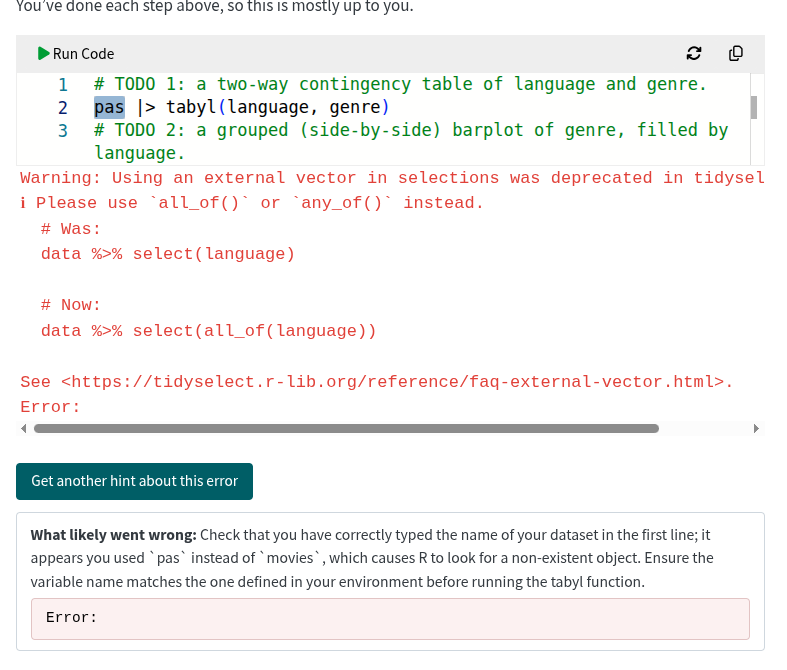
\includegraphics[keepaspectratio]{figures/riegert-llm-1.png}}

}

\subcaption{\label{fig-llm-a}Interpretation of an error}

\end{minipage}%
%
\begin{minipage}{0.50\linewidth}

\centering{

\pandocbounded{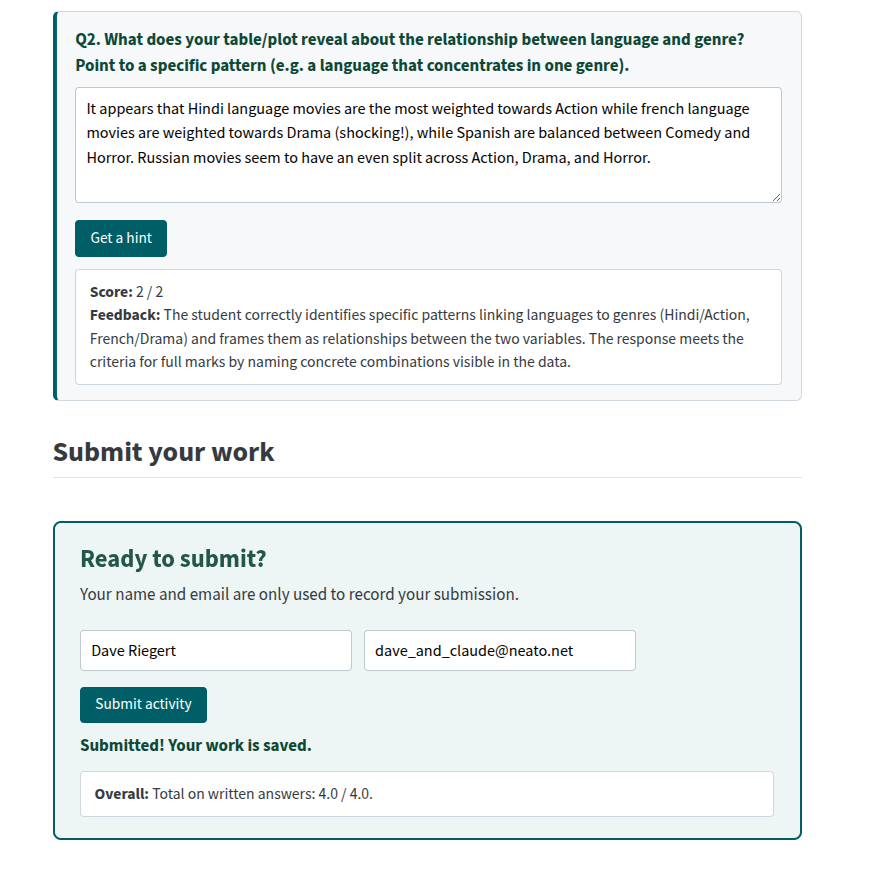
\includegraphics[keepaspectratio]{figures/riegert-llm-4.png}}

}

\subcaption{\label{fig-llm-b}Feedback on a written answer}

\end{minipage}%

\caption{\label{fig-llm}Screenshots of the LLM prototype by D. Riegert,
which is not part of the course skeleton.}

\end{figure}%

\section*{Disclosure statement}\label{disclosure-statement}
\addcontentsline{toc}{section}{Disclosure statement}

N. Mudalige, a co-author of this paper, developed the STA258 tutorial
website (\url{https://nishanmudalige.github.io/STA258_Tutorials/}), from
which the graded tutorial in Figures \ref{fig-exercise} to
\ref{fig-false-positive} is taken. The screenshots of the LLM prototype
in Figure~\ref{fig-llm} were provided by co-author D. Riegert. All other
screenshots were taken from the CanCOTS course skeleton, whose materials
were contributed by the authors.

\section*{Supplementary material}\label{supplementary-material}
\addcontentsline{toc}{section}{Supplementary material}

The source of the course skeleton is available at
\url{https://github.com/nishanmudalige/CanCOTS_2025_Interactive_R_Tutorials},
and the rendered site at
\url{https://nishanmudalige.github.io/CanCOTS_2025_Interactive_R_Tutorials/course_skeleton/index.html}.


\bibliography{references.bib}



\end{document}
